% Created 2021-04-10 sam. 11:50
% Intended LaTeX compiler: pdflatex
\documentclass[a4paper,12pt]{article}
\usepackage[position=top,labelformat=empty]{subfig}
\usepackage{caption}
\usepackage[hmargin=2cm,vmargin=3cm]{geometry}


\usepackage{amsmath}
\usepackage{caption,graphicx}
\usepackage[boxed]{algorithm2e}
\usepackage{authblk,tikz}
\usepackage[left]{lineno}
\linenumbers
\usepackage{setspace}
\doublespacing
\author[]{Vaitea Opuu}
\author[]{Nono S. C. Merleau}
\author[]{Matteo Smerlak}
\affil[]{Max Planck Institute for Mathematics in the Sciences, Leipzig, Germany}
\usetheme{default}
\date{\today}
\title{An RNA fast-folding path heuristic}
\begin{document}

\maketitle
\begin{abstract}
We propose a heuristic to the folding dynamic making use of a mirror encoding
and the fast Fourier transform (FFT) called RAFFT. Based on simple folding
rules, it can create many parallel folding paths. The performance in the folding
task on a well-curated dataset when compared to the state-of-the-art folding
tools was fair. However, when all parallel folding paths were analyzed, it
revealed near-native predictions (79\% PPV and 81\% sensitivity) for sequences of
length below 200 nucleotides. On average, those predictions were found to be of
similar quality to recent deep-learning-based methods. The folding paths were
built with the stem rate model which displays coarse-grained folding paths.
Stems are sequentially added during the folding if it improves the overall
stability. Those two simple rules create smooth coarse-grained folding paths
which are intuitive to analyze and get along with the traditional two states
view of the protein folding landscape. Hence, those paths could well approximate
fast-folding paths. Since the algorithm was designed toward speed, it can
readily be applied to large RNAs.
\end{abstract}

\section*{Introduction}
\label{sec:orgccb777f}
Natural RNA molecules as proteins have biologically relevant functions in many
cellular contexts such as protein translation (mRNA, tRNA\ldots{}), but also in
protein-like functions where RNA can perform enzyme functions. Generally, those
functions can be better understood through the light of their static
tri-dimensional structure. However, some important regulatory RNAs like
riboswitch have their biological function tightly bound to their dynamic
behavior \cite{vitreschak04_ribos}. Therefore, a good understanding of RNAs
dynamical aspects is important.

RNA molecules are bio-polymers composed of nucleotides. These nucleotides are
simple molecules composed of a phosphate-based backbone, a ribose, and a
variable nucleobase. Four different canonical bases/nucleobases compose the RNA,
namely adenine (A), guanine (G), uracil (U), and cytosine (C). As amino-acid
sequences, these nucleotide sequences can form complex tri-dimensional
structures critical for their biological functions. Three main structure types
are generally considered: the primary structure which is the nucleotide sequence
itself. The secondary structure is defined by interacting pairs of nucleobases
called base pairs. Next, the tertiary interactions involve other weaker
non-trivial interactions within the same sequence. Unlike proteins, RNA
structures are usually hierarchically formed. The secondary structure is formed
first, followed by the tertiary structure \cite{tinoco99_how_rna_folds}. Moreover,
the secondary structure provides an accurate enough description of the
thermodynamics and kinetics of RNA molecules. Although base pairs can be formed
with various configurations \cite{leontis01_geomet_nomen_class_rna_base_pairs}, we
considered here only the canonical base pairs edge-to-edge interactions: G-C,
A-U, and G-U. Many subtleties can be used to define the secondary structure, but
we used here a well-accepted formal definition called pseudoknot-free. This
forces the RNA secondary structure to be drawable onto a plan where base pairs
cannot cross. In the res of this work, structure refers to the RNA secondary
structure.

The structure space of an RNA molecule is described by the stability of
individual possible structures. The stability \(\Delta G_s\) of a structure \(s\) is
the free energy changes with the completely unfolded state. To predict secondary
structures, thermodynamic-based methods use empirical data to estimate RNA
stability. By assuming the additivity \cite{dill97_addit_princ_bioch} of the loop
contributions to the overall stability, the nearest-neighbor loop energy model
is the most used model \cite{turner09_nndb}. It is a tabulated set of parameters
associating free energy values, determined by optical melting experiments, to
individual loop types and compositions such as the well known Turner2004 set of
parameters \cite{mathews04_incor_chemic_modif_const_into}. Its functional form
allows for generalizable energy parameters and the use of an efficient dynamic
programming algorithm. It can determine the minimum free energy (MFE) structure
of a sequence in the structure space. The MFE is considered a gold standard for
free-energy-based predictions. Other estimates exist such as the maximum
expected accuracy (MEA), however, it was not found to be significantly better
than the MFE \cite{mathews19_how_to_bench_rna_secon}. Also, the MFE has an
intuitive interpretation. Several tools implement this algorithm, namely Zucker
algorithm \cite{zuker81_optim_comput_foldin_large_rna}, such as RNAfold
\cite{hofacker03_vienn_rna_secon_struc_server}, Mfold
\cite{zuker03_mfold_web_server_nucleic_acid}, or RNAstructure \cite{reuter10_rnast}.
Although those methods were found to be consistently accurate at predicting RNA
secondary structures as shown in recent benchmarks
\cite{sato20_rna,huang19_linear}, the additivity foundation is expected to be
doomed when sequences get larger and structures complexify. The non-additivity
of tertiary interactions and pseudoknots pairings can partially explain this
discrepancy. Pseudoknots loop are not defined in the main parameters sets like
the Turner2004 model. Another limit of such structure estimates is the static
picture that it gives to the RNA folding landscape. From a dynamical standpoint,
the sequence navigates the structure space by following the landscape drawn by
the stability.

Dynamical information on RNA molecules was found to give valuable complementary
information. To follow the dynamic of individual RNA molecules, three rate
models describing elementary steps in the structure space are currently used.
The base stack model uses base stacks formation and breaking as elementary moves
. The base pair rate model uses base pairs as elementary steps as implemented in
kinfold \cite{flamm00_rna_foldin_at_elemen_step_resol}. kinfold uses a
continuous-time Monte Carlo simulation to follow the RNA folding. It gives the
finest resolution in the secondary structure folding landscape, but at the cost
of computation time. The stem model uses the creation or deletion of stems to
construct the folding dynamics. It is the first strategy explored
\cite{martinez84_rna_foldin_rule}, and provides a coarse-grained description of
the kinetic. The folding rates are determined by the free energy changes when
stems are added or removed. Although none of these models were definitively
rejected nor accepted, this one makes a notable assumption. Indeed, transition
states (or saddle points) hidden in the formation of a given stem are not
considered. An alternative approach, implemented in kinwalker
\cite{geis2008folding}, used the observation that folded intermediates are
generally locally optimal conformations. Therefore, locally optimal structures
are formed using the standard dynamic programming algorithm and aggregated
together along with the folding dynamic.

From folding experiments, Pan and coworkers found parallel pathways for a
ribozyme which involve two types of path to reach the native structure
\cite{pan97_foldin_rna_invol_paral_pathw}. One population of sequences was found
to fold rapidly, and one quickly reached metastable misfolded structures that
slowly fold into the native structure. It is a direct consequence of the
rugdness nature of the RNA folding landscape
\cite{solomatin10_multip_nativ_states_reveal_persis}. Russell and coworkers
revealed experimentally the presence of deep channels separated by large energy
barriers on the folding landscape which lead to the fast and slow folding paths
observed \cite{russell01_explor_foldin_lands_struc_rna}.

Here we propose a complementary approach by approximating fast-folding paths
based on simple folding rules. The basic idea is to use the stem rate model to
create multiple parallel folding paths. Here, stems are not allowed to be
removed and can be formed only if it improves the stability. It uses a mirror
encoding and relies on the fast Fourier transform to speed up the search of
stems. This method is inspired by MAFFT \cite{katoh02_mafft}, a well-known
multiple-sequence-alignment tool. The mirror encoding is a simple numerical
orthogonal representation of nucleotide sequences. Other similar encodings
combined with the FFT were developed for the analysis of DNA
\cite{felsenstein82_effic_method_match_nucleic_acid_sequen}. To assess the
reliability of the paths predicted, we compared its performance on the folding
task for a well-curated dataset, archive II
\cite{mathews19_how_to_bench_rna_secon}. The algorithm is compared to two
estimates: the MFE computed by RNAfold and an ML estimate computed with MxFold2,
a recent deep-learning based method \cite{sato20_rna}. Next, we applied the
algorithm to a simple test case, the Coronavirus frameshifting stimulation
element \cite{baranov05_progr_ribos_frames_decod_sars_cov_genom}, where it
found closer structures than the MFE.

\section*{FFT based folding dynamic heuristic}
\label{sec:org3f46004}
We now describe the heuristic starting from one sequence S and its associated
unfolded structure of length L. We first create a numerical representation of S
where each type of nucleotide is replaced by a unit vector of 4 components:
\begin{equation}
\begin{split}
A \rightarrow \begin{pmatrix} 1 0 0 0 \end{pmatrix}
U \rightarrow \begin{pmatrix} 0 0 0 1 \end{pmatrix}
C \rightarrow \begin{pmatrix} 0 1 0 0 \end{pmatrix}
G \rightarrow \begin{pmatrix} 0 0 1 0 \end{pmatrix}
\end{split}
\end{equation}
which gives us a \(4 \times L\) matrix we call \(X\) where each row is a nucleotide
type channel. Here, the first row would be the A channel which we refer to as
\(X^A\). Then, we create a second copy for which we revert the order of the
sequence and use the following complementary encoding:
\begin{equation}
\begin{split}
\bar{A} \rightarrow \begin{pmatrix} 0 0 0 w_{\scalebox{0.5}{AU}} \end{pmatrix}
\bar{U} \rightarrow \begin{pmatrix} w_{\scalebox{0.5}{AU}} w_{\scalebox{0.5}{GU}} 0 0 \end{pmatrix}
\bar{C} \rightarrow \begin{pmatrix} 0 0 w_{\scalebox{0.5}{GC}} 0 \end{pmatrix}
\bar{G} \rightarrow \begin{pmatrix} 0 w_{\scalebox{0.5}{GC}} 0 w_{\scalebox{0.5}{GU}} \end{pmatrix}
\end{split}
\end{equation}
Where \(\bar{A}\) (respectively \(\bar{U}, \bar{C}, \bar{G}\)) is the complementary
of \(A\) (respectively \(U, C, G\)). \(w_{AU}\), \(w_{GC}\), \(w_{GU\) are tunable
parameters for the next step. We call this new complementary copy \(\bar{X}\), the
mirror of \(X\).

Next, for each of the 4 channels, we compute the correlation between \(X\) and
\(\bar{X}\) and by simply summing up the channel correlations, we obtain the
correlation between the two copies:
\begin{equation}
cor(k) = (c_{X^A,\bar{X}^A}(k) + c_{X^U,\bar{X}^U}(k) + c_{X^G,\bar{X}^G}(k) + c_{X^C,\bar{X}^C}(k)) / min(k, 2 \times L-k)
\end{equation}
where \(c_{X^A,\bar{X}^A(k)\) is the correlation in the \(A\) channel between the
two copies. \(cor(k)\) gives the average number of base pairs for a positional lag
\(k\). One channel correlation between copies is given by:
\begin{equation}
c_{X^A,\bar{X}^A}(k) = \sum\limits_{1\leq i \leq L, 1 \leq i + k \leq M} X^A(i) \times \bar{X}^A(i+k)
\end{equation}
where \(X^A(i)\) and \(\bar{X}^A(i+k)\) are the A channel of site \(i\) and \(i+k\).
\(X^A(i) \times \bar{X}^A(i+k)\) is non zero if sites \(i\) and \(i+k\) can form a
base pair, and will have the value of the chosen weight as described above.
Although this requires \(O(N^2)\) operations, it can take advantage of the FFT
which reduces drastically its complexity to \(O(Nlog(N))\).

The large correlation values between the two copies indicate the positional lag
at which the base pair density is high. Therefore, we use a sliding window
strategy to search for the longest consecutive base pairs within the positional
lag. Since the copies are symmetrical, we only need to slide over one-half of
the positional lag. Once the longest base pairs are identified, we simply
compute the free energy change when those base pairs are formed. We perform the
same search for the \(n\) highest correlation lags, which gives us \(n\) potential
stems. Then, we add to the current structure the base pairs that give the best
change of free energy. Free energies were computed using Turner 2004 energy
parameters through Vienna RNA package API \cite{lorenz11_vienn_packag}.

We are now left with two segments, the interior, and exterior of the group of
consecutive base pairs formed. The two exterior fragments are concatenated
together. Then, we simply apply recursively the same procedure on the two
segments separately in a "Breadth First" fashion to form new consecutive base
pairs, until no base pair formation can improve the energy. Hence, it is
straightforward to consider pseudoknots by simply concatenating all the
fragments left. When multiple stems can be formed in these independent
fragments, we combine those possible independent stems and pick the composition
that has the best overall stability.

The algorithm described so far tends to be stuck in the first local minima found
along the folding trajectory. To alleviate this, we propose a stacking procedure
where the best trajectories are stored in a stack and evolved in parallel.
Hence, it offers the flexibility of overcoming some energy barriers. Once no
stem can be formed, the algorithm stops and output the structure with the best
energy found among the structures saved in the stack.

\section*{Application to the folding task}
\label{sec:orgbf52117}
To evaluate the relevance of the folding dynamic heuristic, we compared its
performance for the folding task. Also, to assess the effect of sequence
lengthens on these predictions, we analyzed their performance length-wise. To
localize its performance, we compared with two estimates: the MFE structure
computed by RNAfold and the ML-based structure computed by MxFold2. RAFFT
predictions were performed using non-optimized weights. 50 structures are formed
in parallel for each sequence and 100 positional lags were explored at each step
for each of the 50 structures.

Figure \ref{perf_fig} shows the performance in predicted positive values (PPV) and
sensitivity for the three methods. It shows that the ML method is consistently
better than thermodynamic-based methods. Length-wise T-test between the MFE and
ML predictions showed that this difference is significant (p-value \(\approx\)
10\textsuperscript{-12}) with a substantial improvement of about 10\%. Although RAFFT
predictions were found to be comparable to MFE predictions, they are
significantly less accurate (p-value \(\approx\) 0.0002), with a drastic loss of
performance for sequences of length greater than 300 nucleotides.

Among the 50 structures produced by RAFFT, we found on average at least one
prediction with 59\% of PPV and 63\% of sensitivity as shown figure \ref{perf_fig}.
The overall gain of performances is not significantly different from the MFE
predictions. However, for the sequences of length below 200 nucleotides, this
gain was found to be substantial and significant (\(\approx\) 16 \% better than the
MFE) with PVV \(\approx\) 79\% and sensitivity \(\approx\) 81\%. The accuracy for those
sequences is equivalent to ML performances. For sequence lengths greater than
300 nucleotides, we observed the same drastic loss of accuracy, although we took
only the best prediction among the 50 saved configurations for each sequence. We
investigated the dependency to the base pair spanning, however, we did not find
any significant effect (see supp. mat.).

Two regions of lack of performance were observed for all methods. A group of 28
sequences of length shorter than 80 nucleotides have their known structures at
on average 9.8 kcal/mol greater than the MFE structures. Some of them involve
large unpaired loops such as displayed in figure \ref{diff_struct}. The second
region is around 200 nucleotides in length. The known structure of those
sequences also displayed large unpaired regions \ref{diff_struct}.

\begin{figure}[!ht]
  \centering
  \subfloat[]{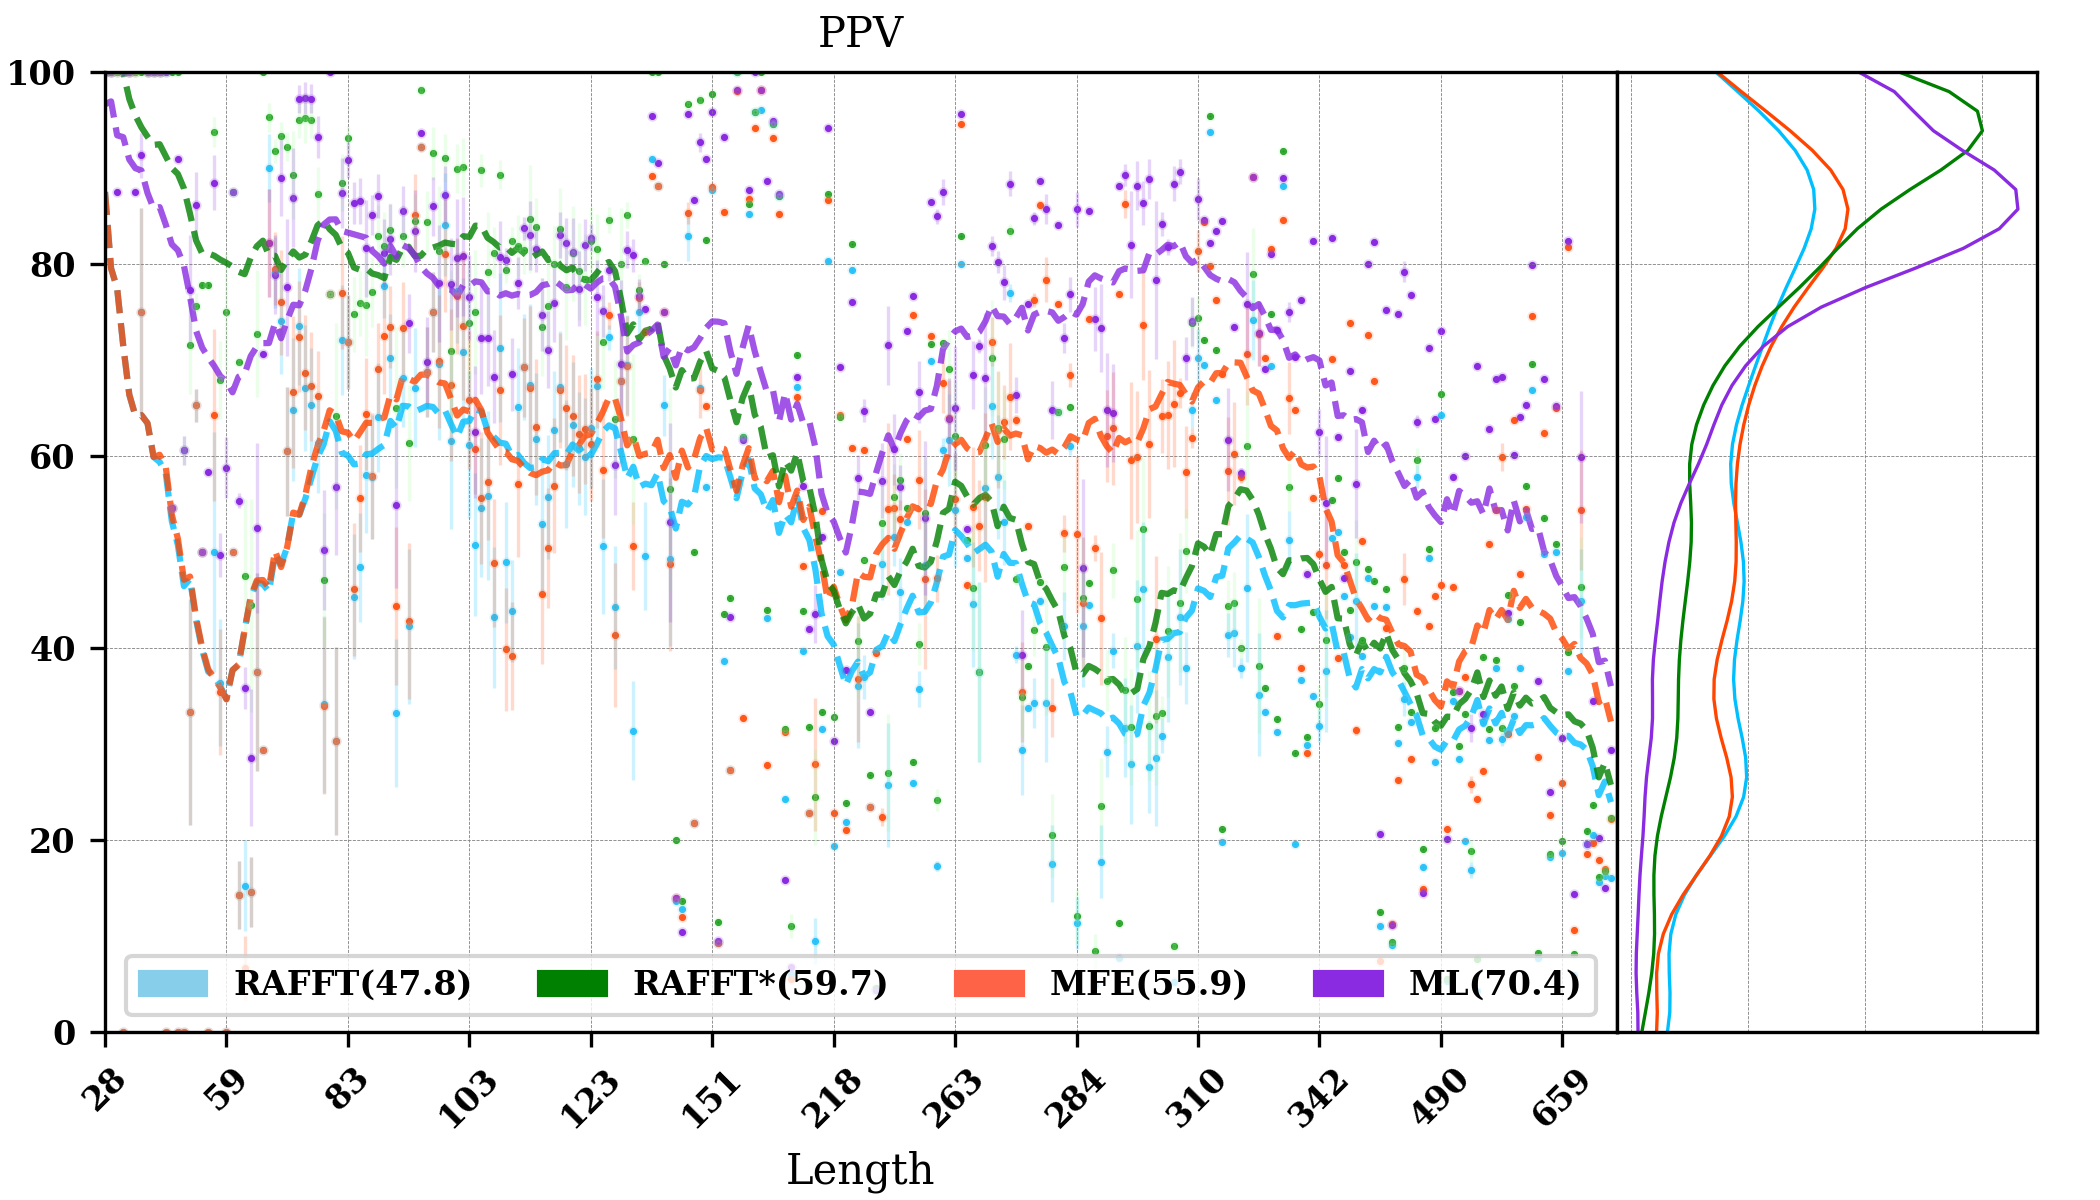
\includegraphics[scale=0.5]{img/fold_perf_ppv.png}}\\
  \subfloat[]{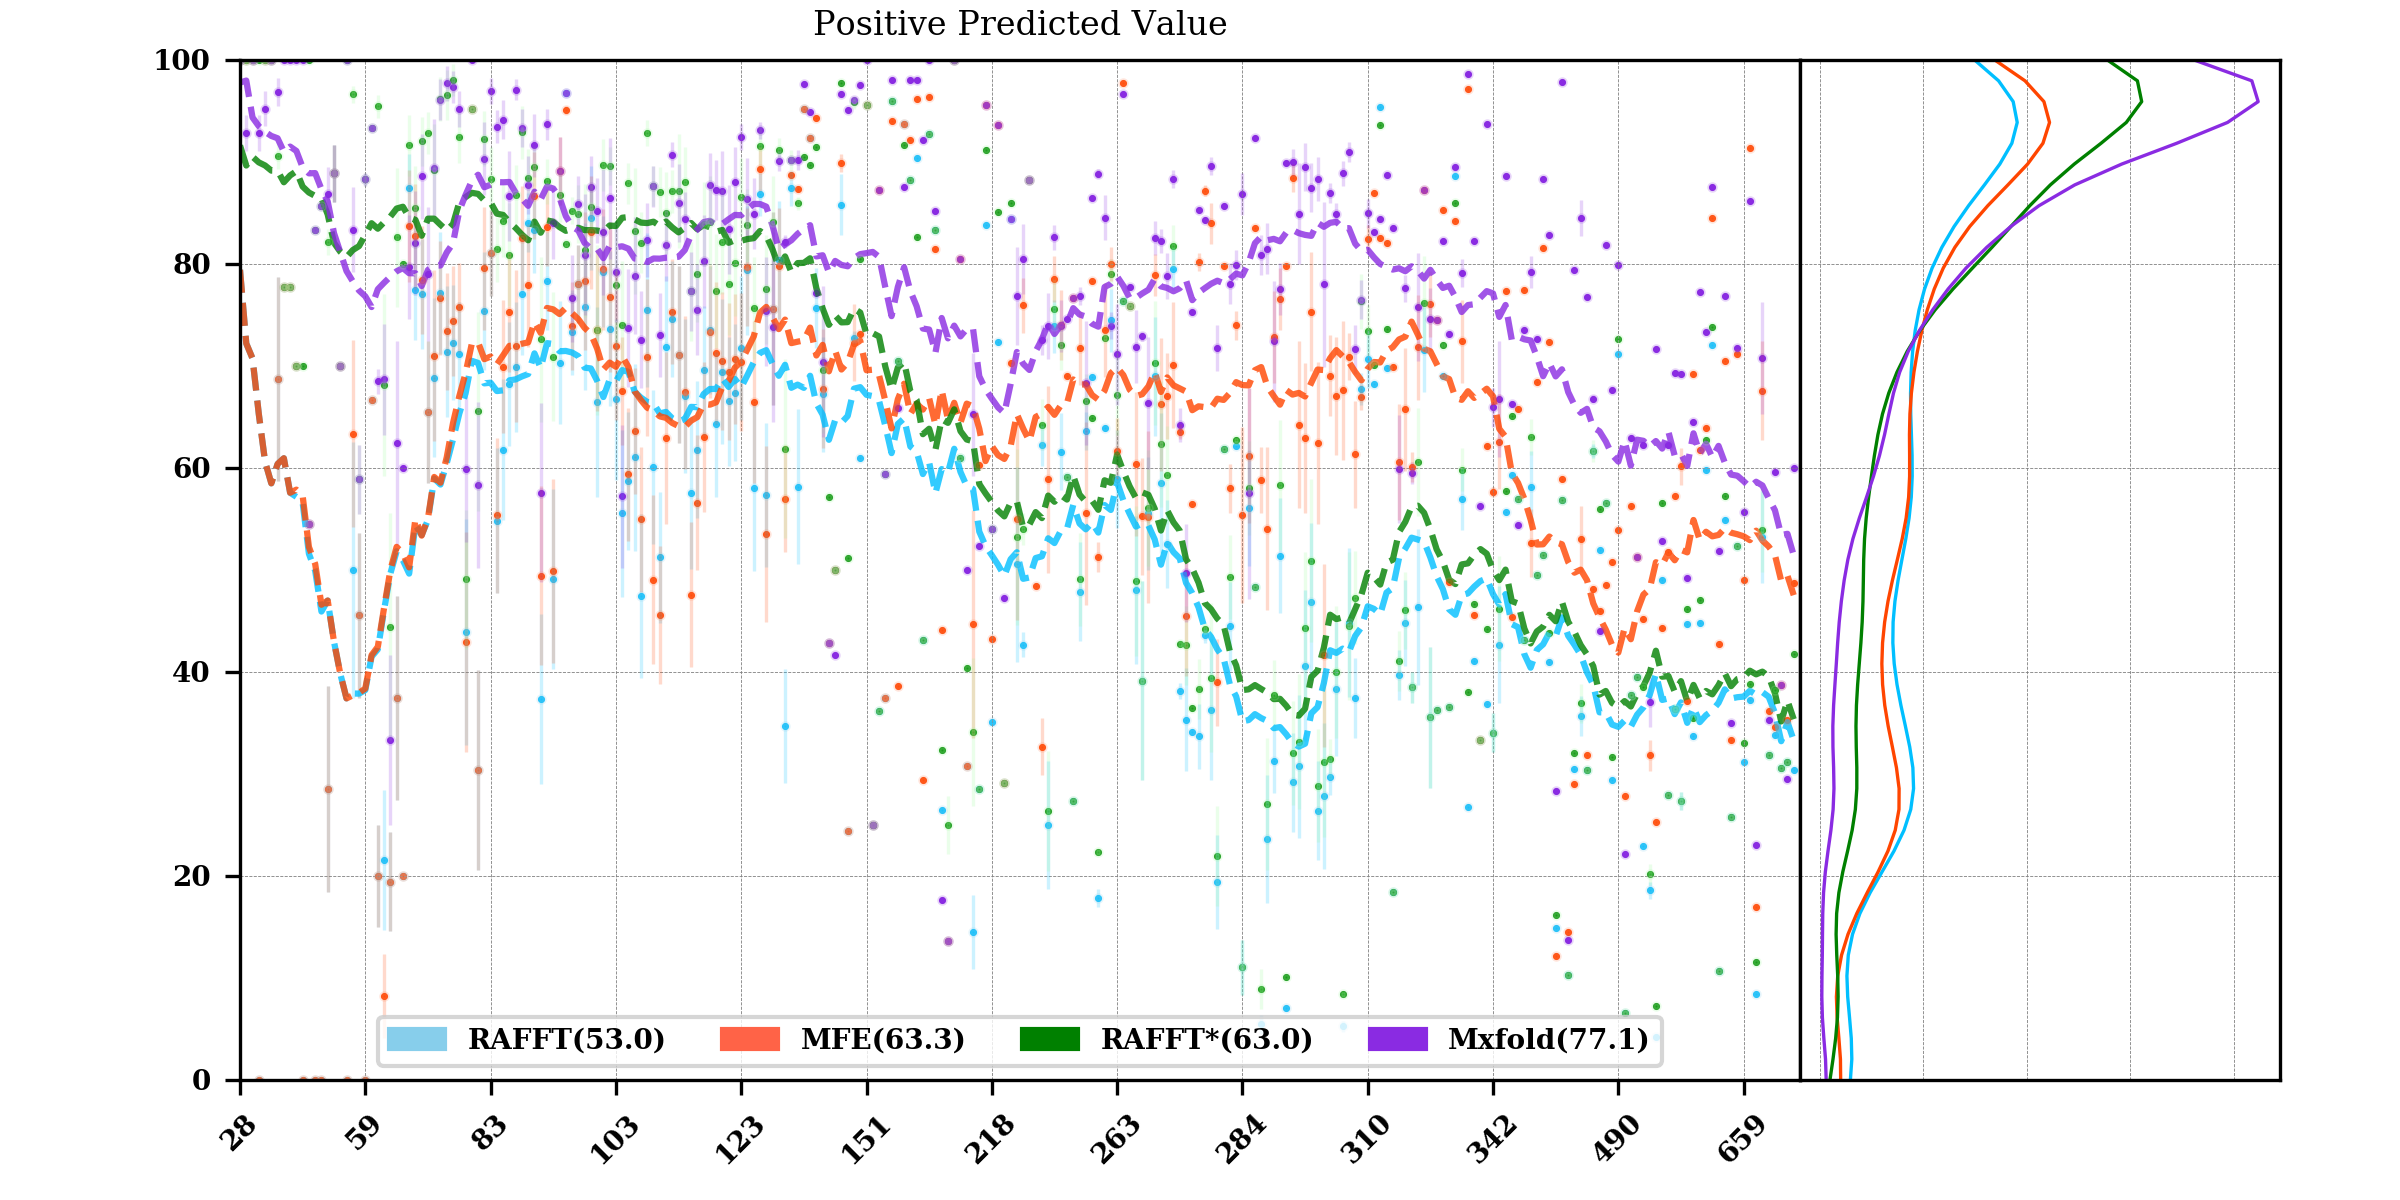
\includegraphics[scale=0.5]{img/fold_perf_sens.png}}
  \caption{\textbf{Predicted positive values and sensitivity
      results\label{perf_fig}.} RAFFT (blue) displayed the best energy found.
    RAFFT* shows the best score found among 50 saved structures. Right pans show
    the density (sequence-wise) of the accuracy measures.}
\end{figure}

\begin{figure}[!ht]
  \centering
  \subfloat[\texttt{srp\_Synt.wolf.\_CP000448}]{
  \begin{tikzpicture}
    \node (s11) at (0cm,3cm) {\subfloat[RAFFT]{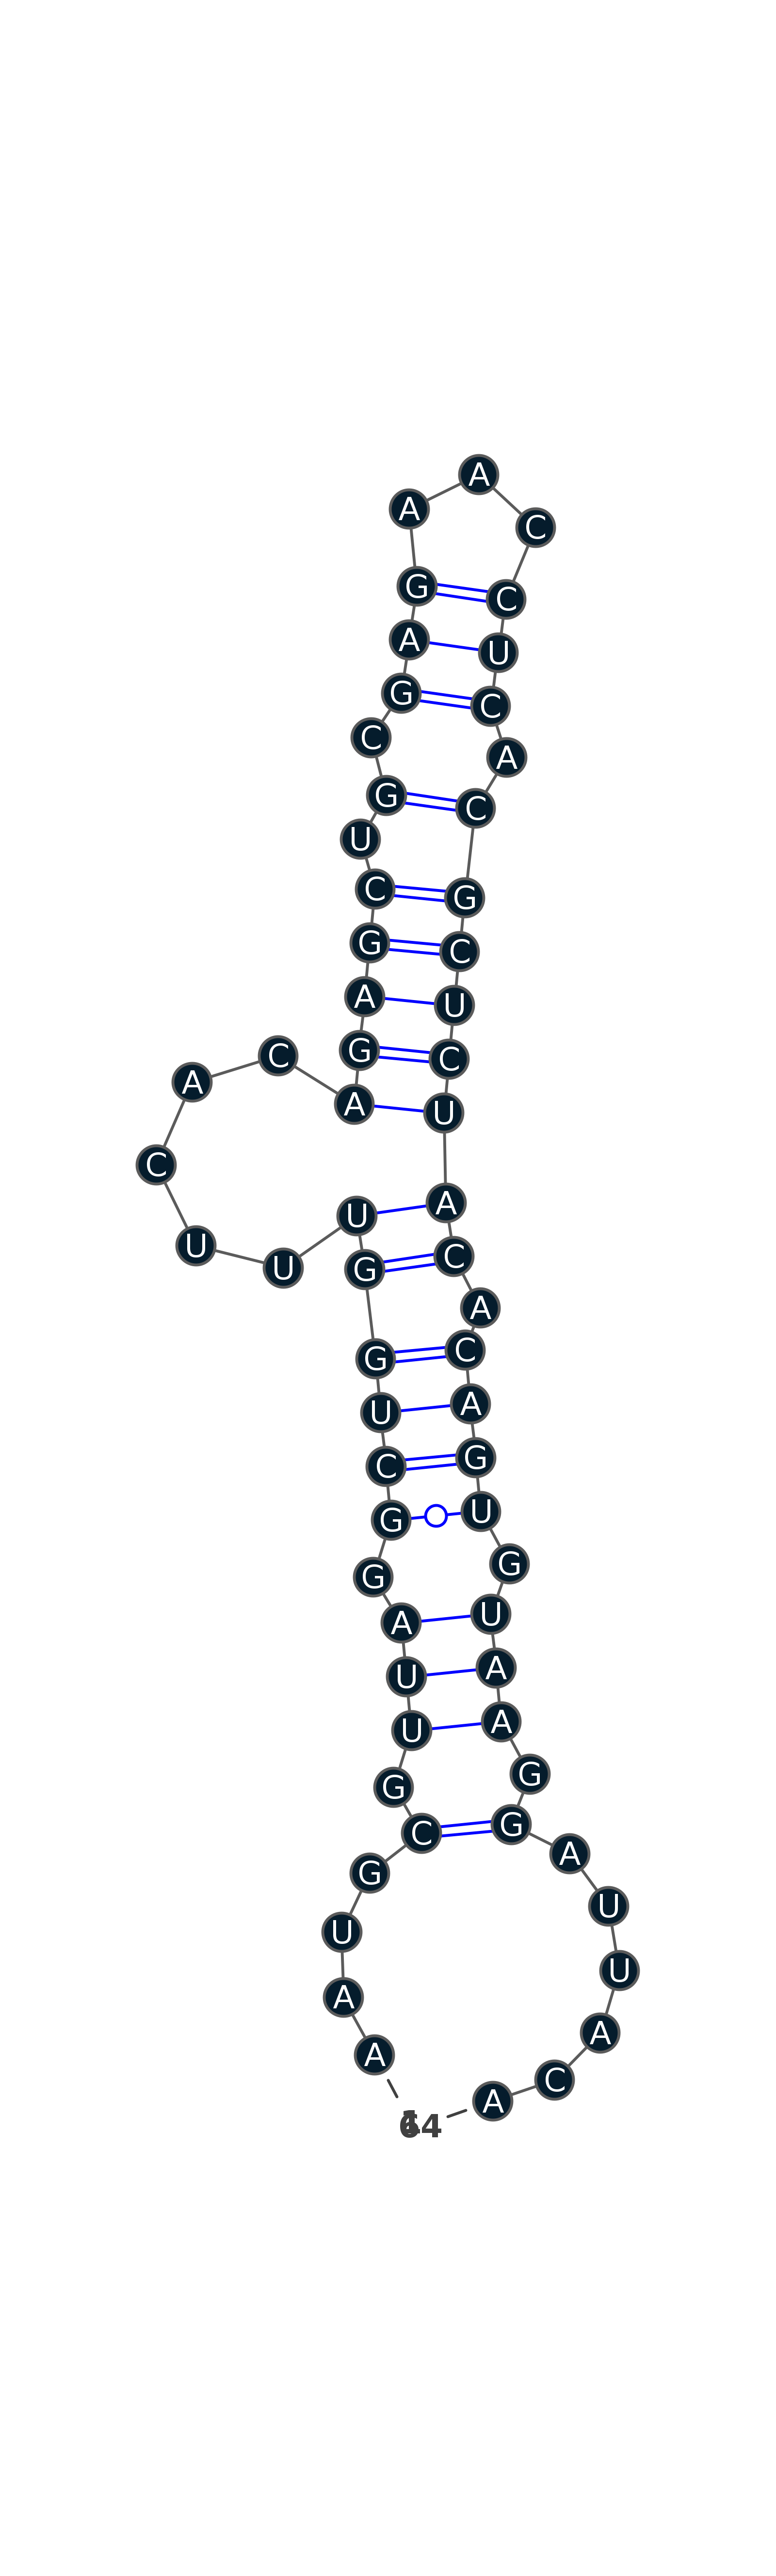
\includegraphics[scale=0.05]{./img/illed_img/srp_Heli_fft.png}}};
    \node (s12) at (3cm,3cm) {\subfloat[MFE]{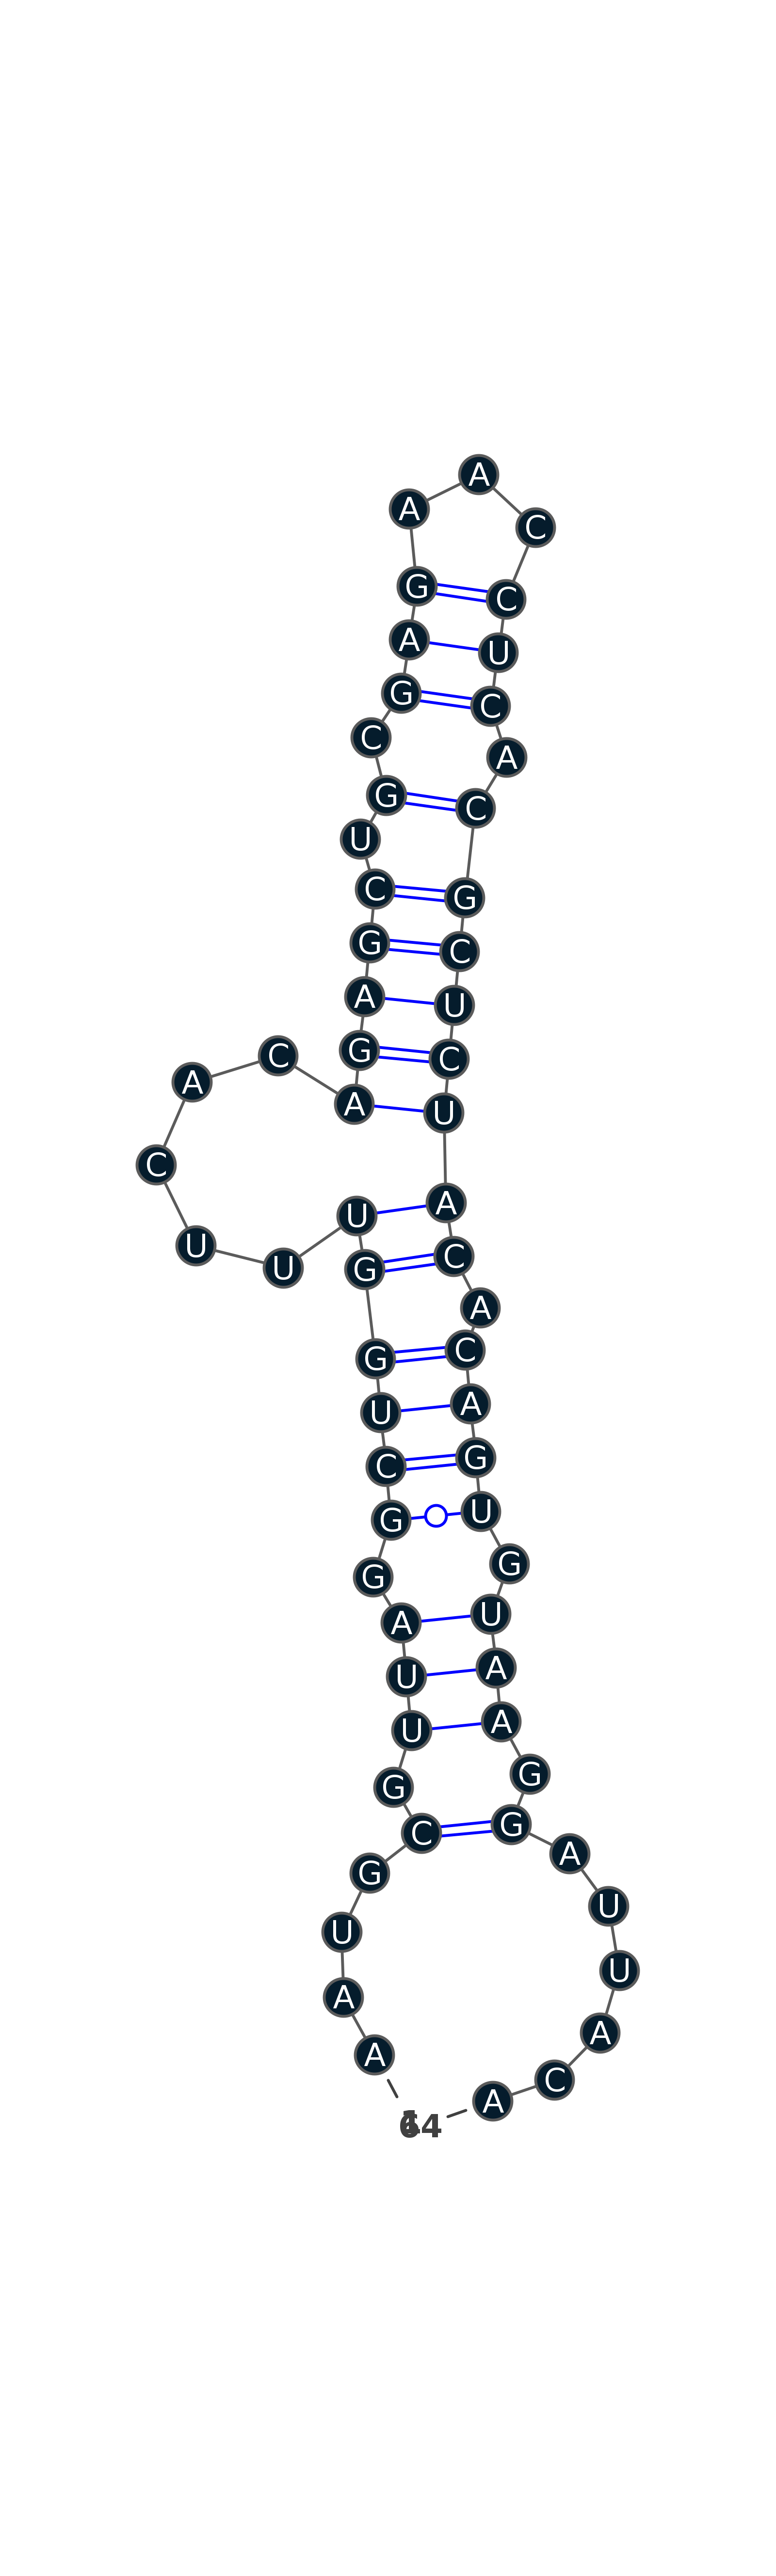
\includegraphics[scale=0.05]{./img/illed_img/srp_Heli_mfe.png}}};
    \node (s13) at (0cm,0cm) {\subfloat[ML]{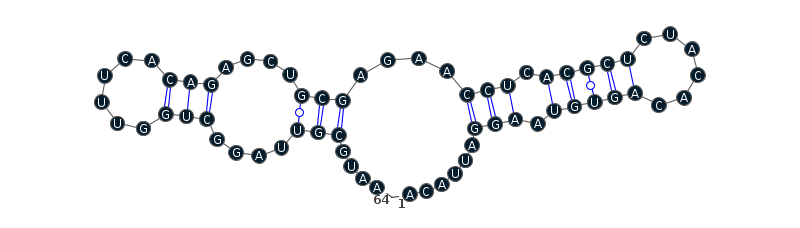
\includegraphics[scale=0.09]{./img/illed_img/srp_Heli_mle.png}}};
    \node (s14) at (3cm,0cm) {\subfloat[WT]{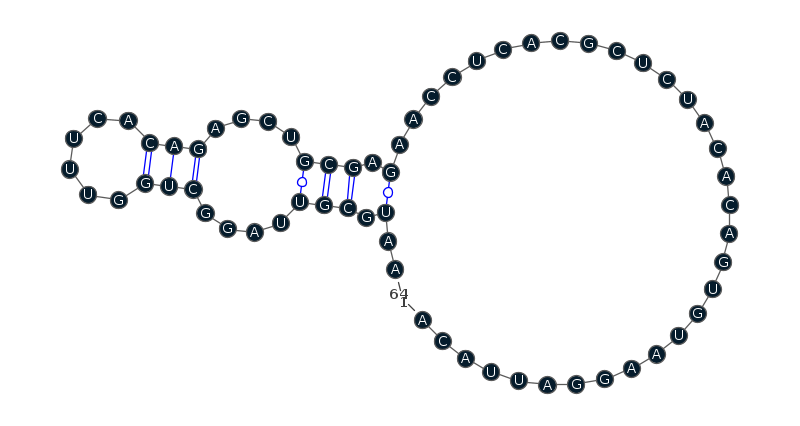
\includegraphics[scale=0.09]{./img/illed_img/srp_Heli_wts.png}}};
  \end{tikzpicture}
  }
  \subfloat[\texttt{srp\_Meth.mari.\_CP000745}]{
  \begin{tikzpicture}
    \node (s11) at (0cm,3cm) {\subfloat[RAFFT]{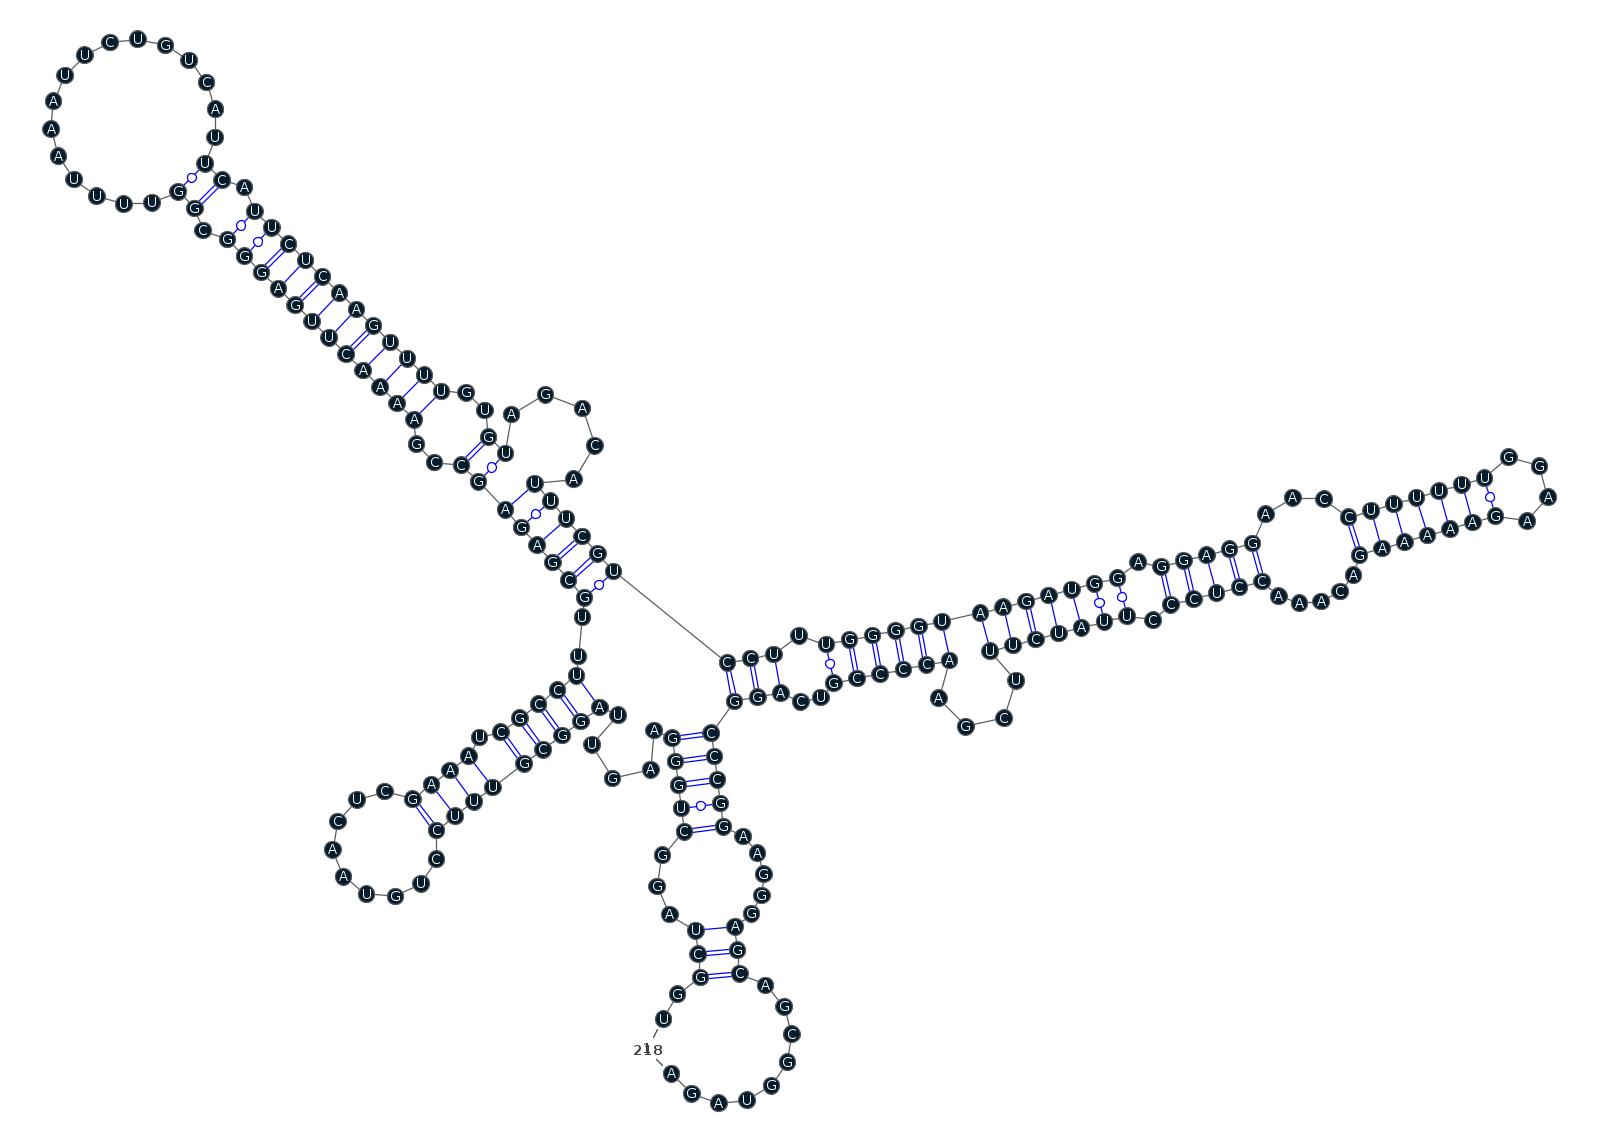
\includegraphics[scale=0.10]{./img/illed_img/srp_Meth_fft.png}}};
    \node (s12) at (3cm,3cm) {\subfloat[MFE]{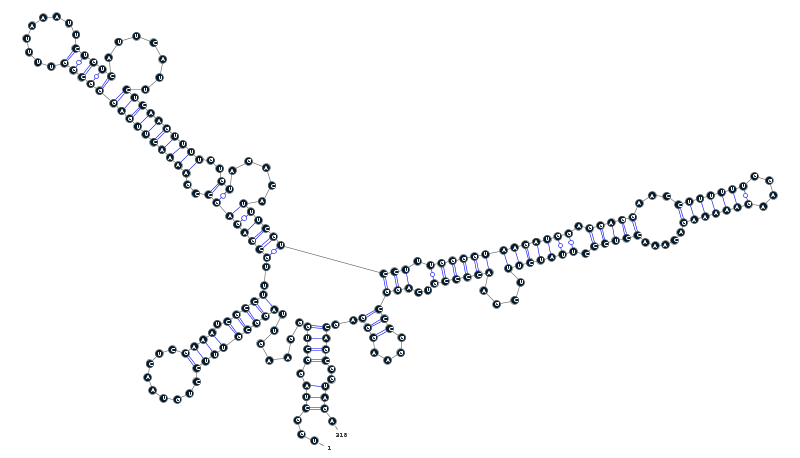
\includegraphics[scale=0.10]{./img/illed_img/srp_Meth_mfe.png}}};
    \node (s13) at (0cm,0cm) {\subfloat[ML]{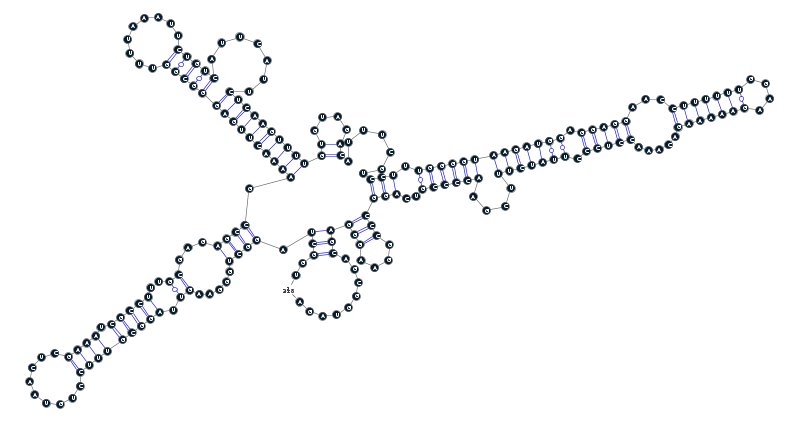
\includegraphics[scale=0.10]{./img/illed_img/srp_Meth_mle.png}}};
    \node (s14) at (3cm,0cm) {\subfloat[WT]{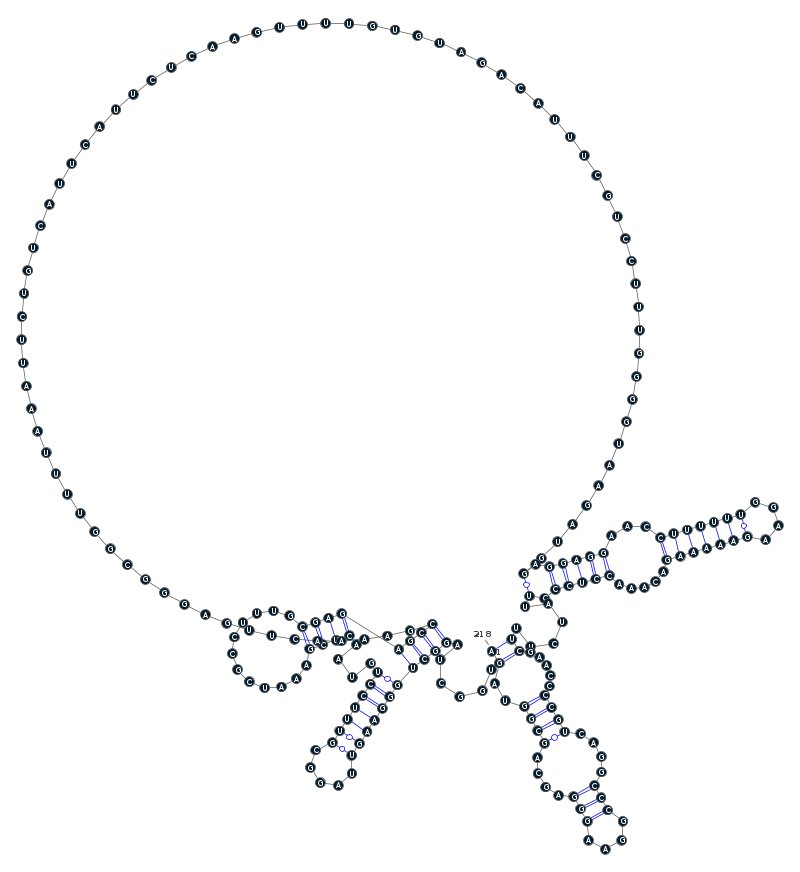
\includegraphics[scale=0.10]{./img/illed_img/srp_Meth_wts.png}}};
  \end{tikzpicture}
  }\\
  \subfloat[\texttt{tmRNA\_Cyan.mero.\_AY286123\_1\-236}]{
  \begin{tikzpicture}
    \node (s11) at (0cm,0cm) {\subfloat[RAFFT]{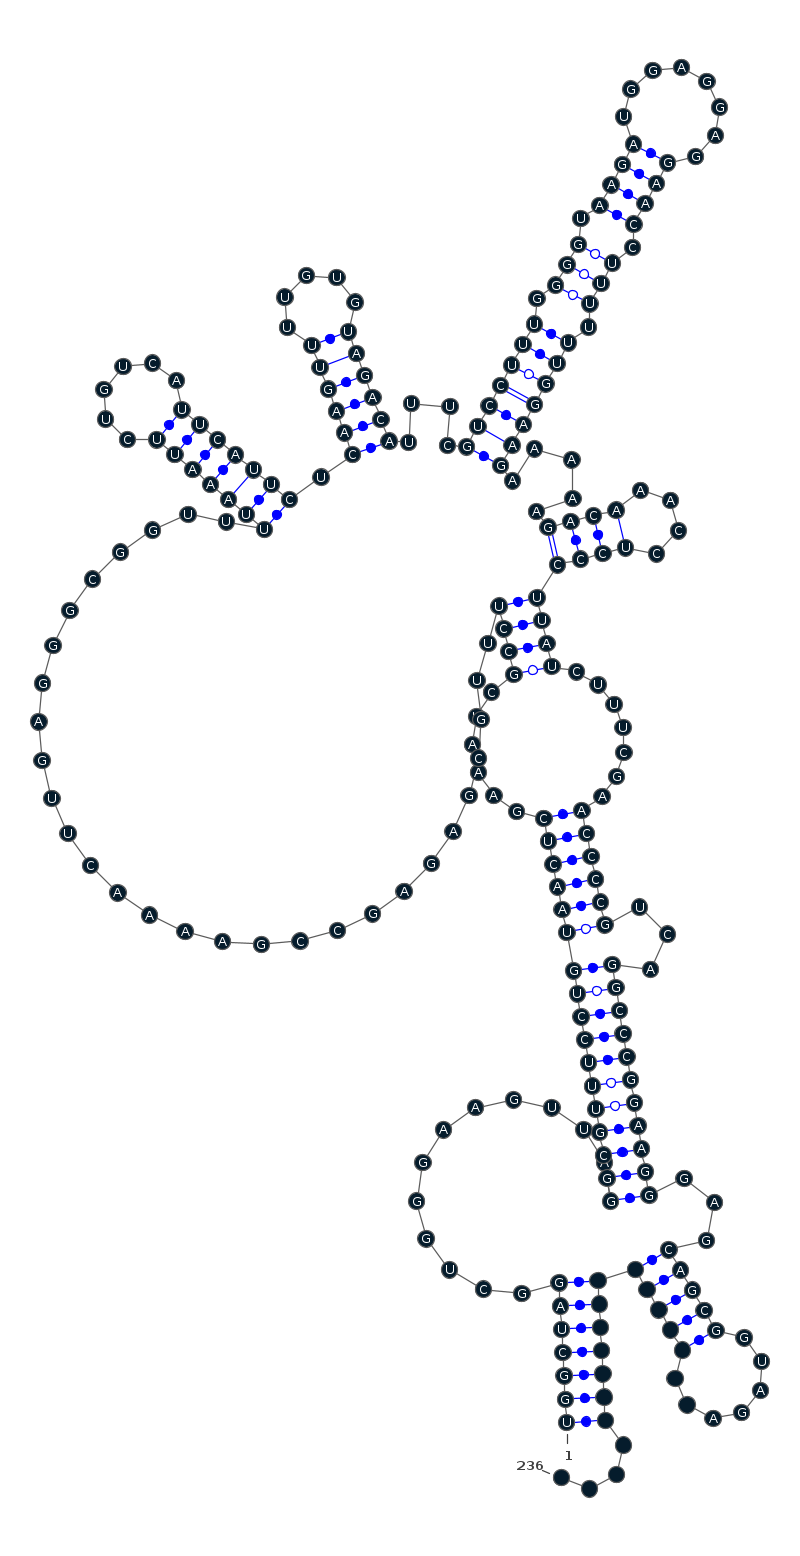
\includegraphics[scale=0.08]{./img/illed_img/tmRNA_Cyan_fft.png}}};
    \node (s12) at (3cm,0cm) {\subfloat[MFE]{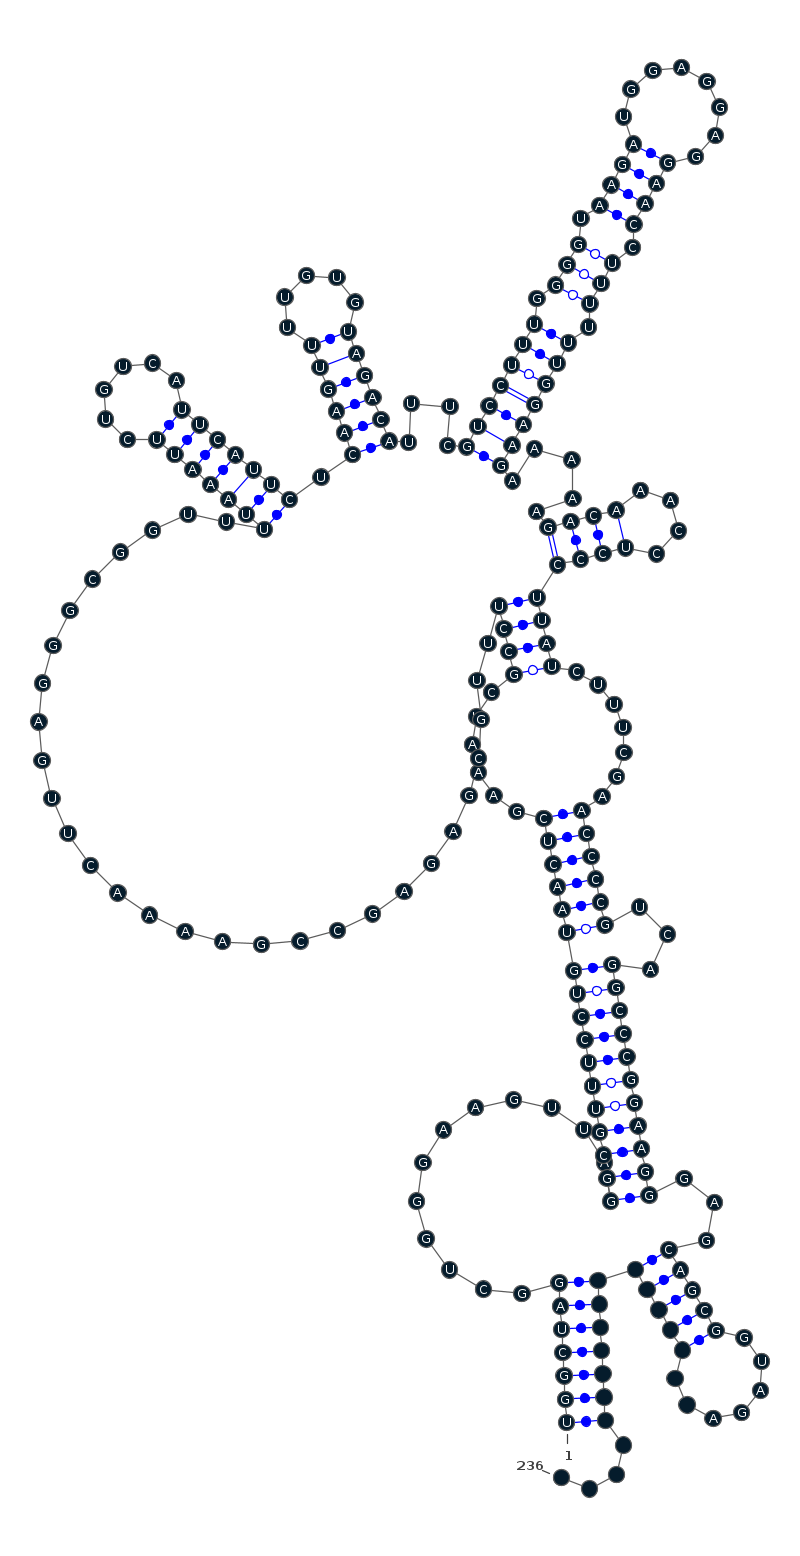
\includegraphics[scale=0.08]{./img/illed_img/tmRNA_Cyan_mfe.png}}};
    \node (s13) at (6cm,0cm) {\subfloat[ML]{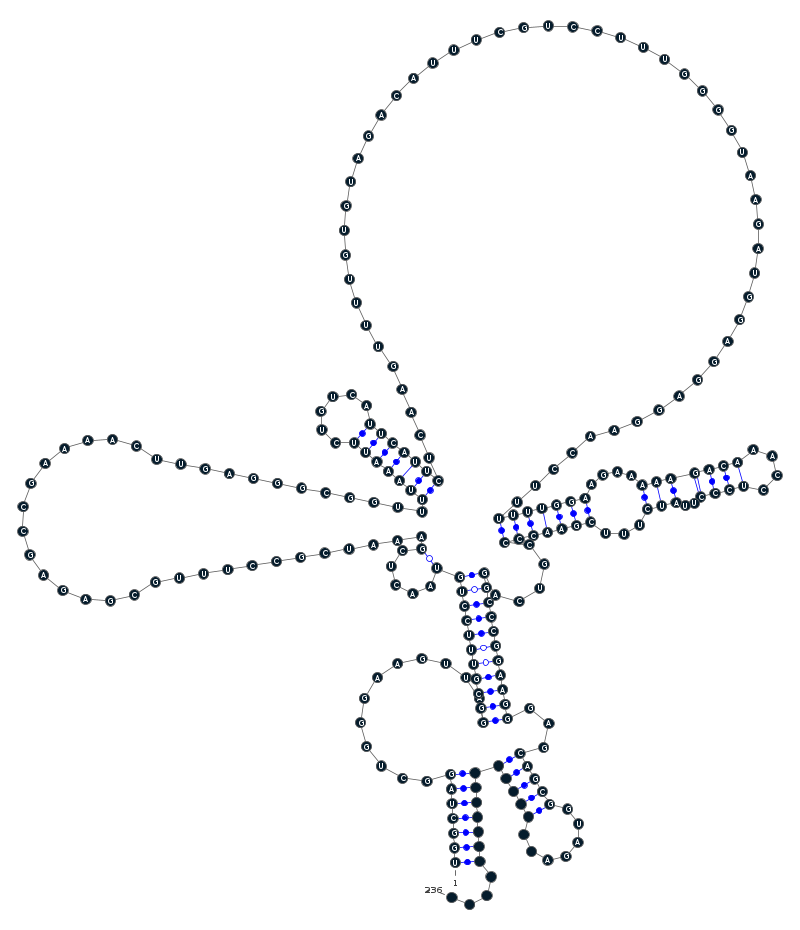
\includegraphics[scale=0.1]{./img/illed_img/tmRNA_Cyan_mle.png}}};
    \node (s14) at (9cm,0cm) {\subfloat[WT]{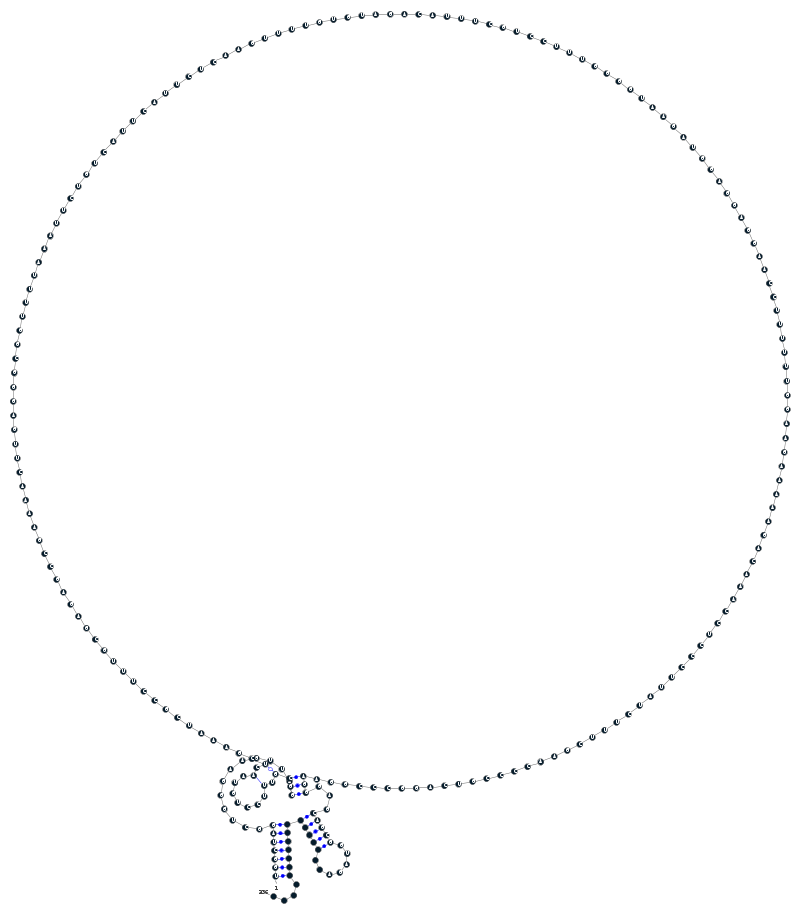
\includegraphics[scale=0.1]{./img/illed_img/tmRNA_Cyan_wts.png}}};
  \end{tikzpicture}
  }

  \caption{\textbf{Structures found to be difficult to predict with the
      thermodynamic model.} The sequence name where extracted directly from the
    dataset. WT is the known structure.\label{diff_struct}}
\end{figure}

To investigate the region of the structure space where the thermodynamic model
tends to fail, we computed the composition of the known structures. Loop type
lengths were computed in percents. Figure \ref{pca_struct} shows principal
component analysis (PCA) of those compositions. From the PCA, we observed that
the known structures are distributed in the structure space toward interior
loops. Also, some natural structures, as shown in figure \ref{diff_struct}, have
large unpaired loops. The center of mass in the principal component space is
located in between the high-density stacking and interior loops. This shows that
the dataset contains many elongated structures.

Next, we investigated the structure space produced by the three methods. The
thermodynamic approach seems to produce a more diverse structure space as shown
in figure \ref{pca_struct}. Loop contents were extracted from the predicted
structures of each method and projected onto their respective two first
principal components space. Both RAFFT and MFE predictions seem to produce
similar structure spaces while the ML method does allow for long unpaired
regions in long hairpins which tend to be closer to the dataset structure space.

\begin{figure}[!ht]
  \centering
  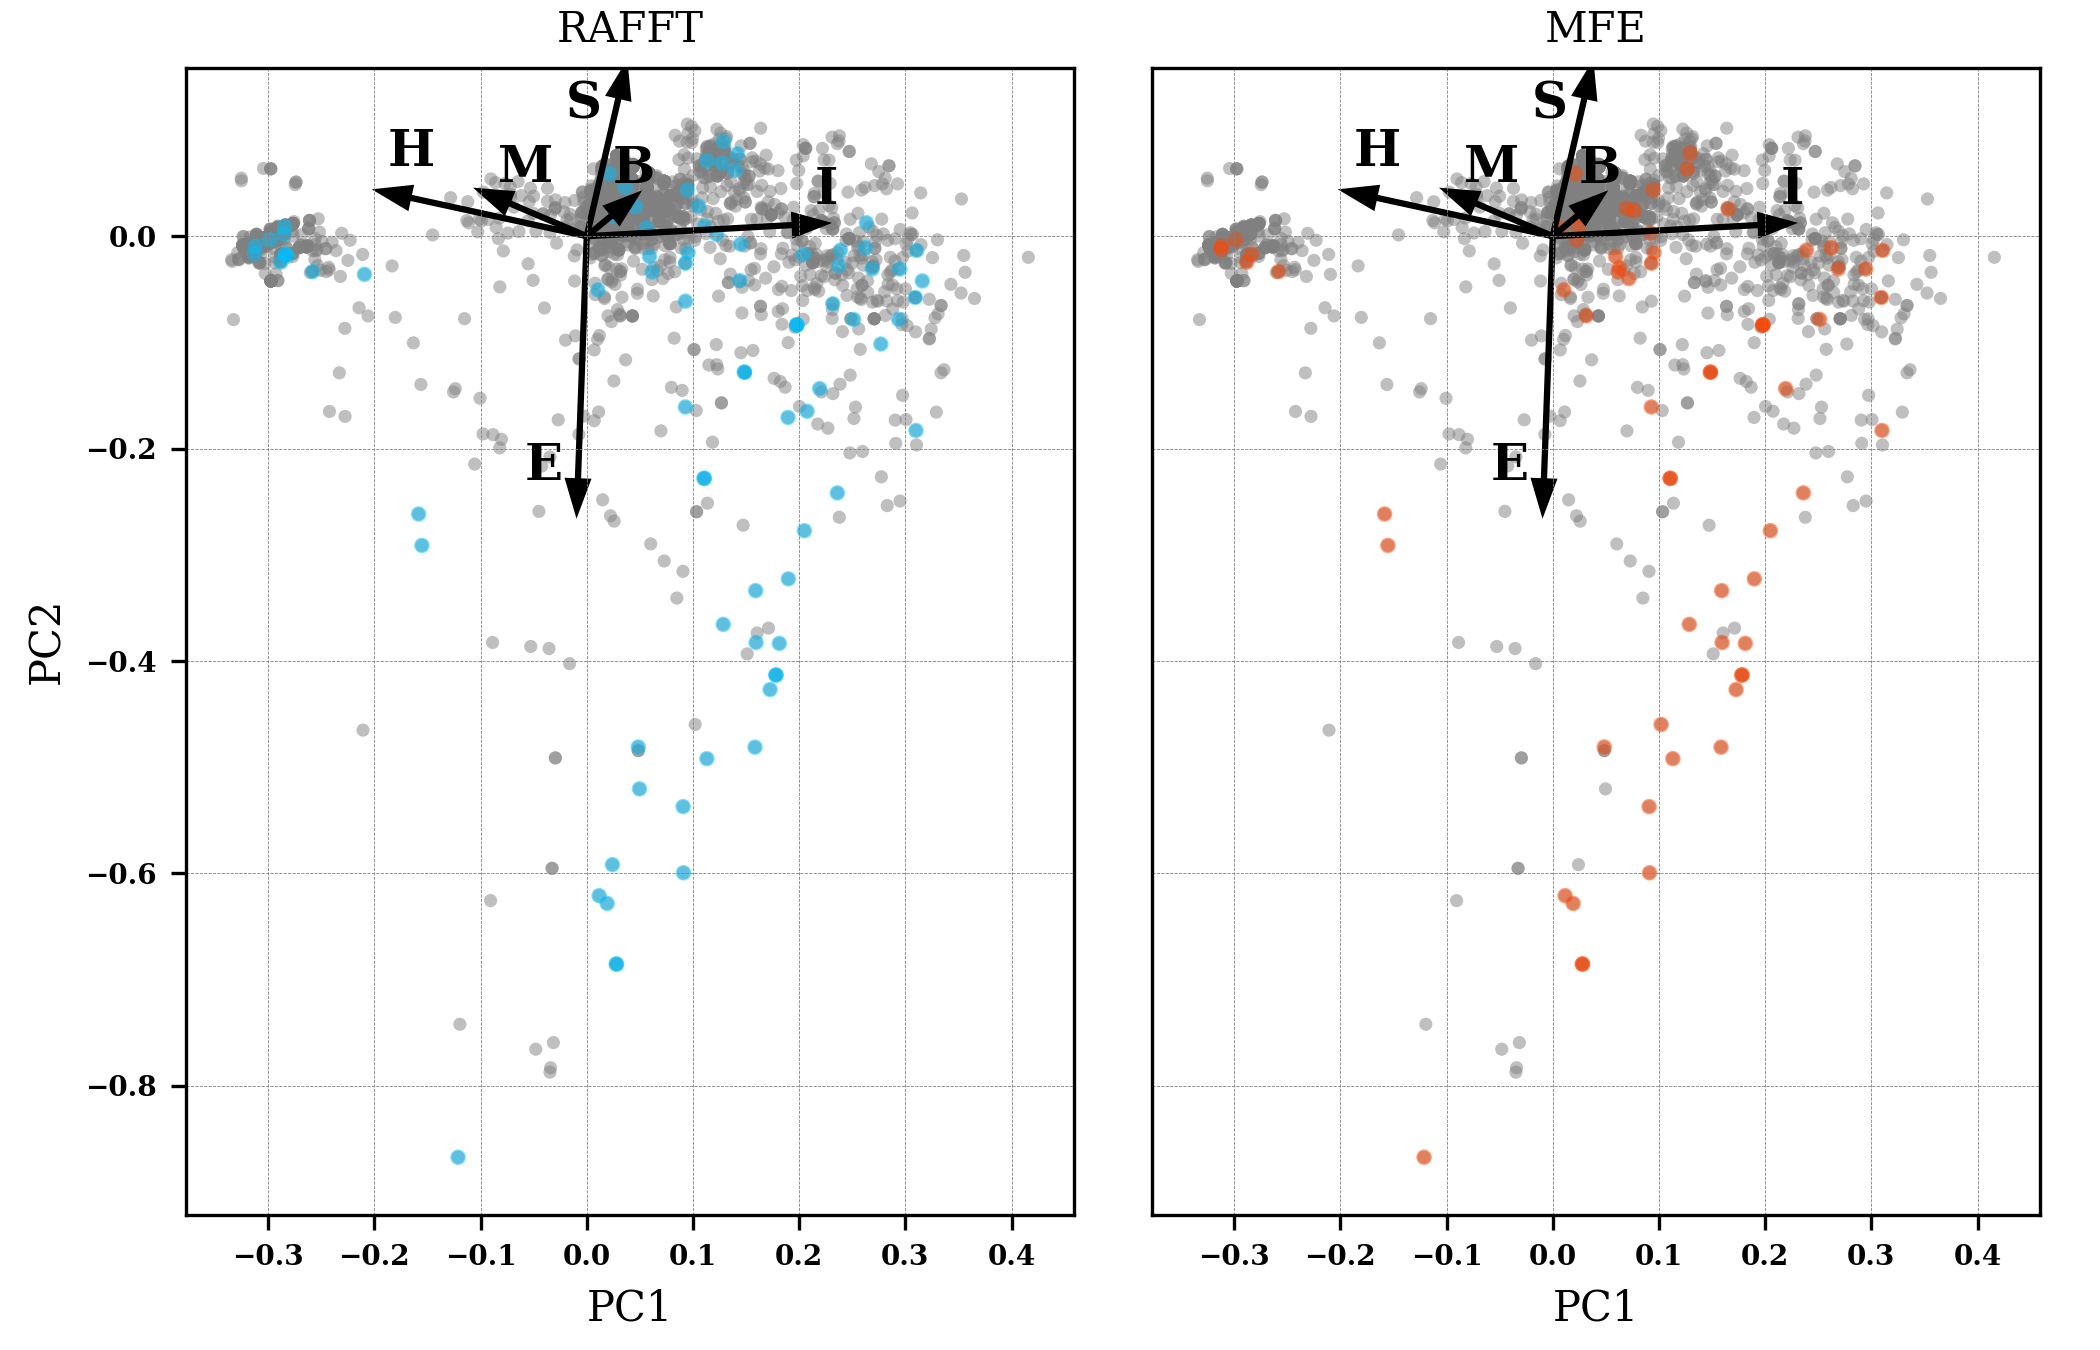
\includegraphics[scale=0.6]{img/pca_known.png}\\
  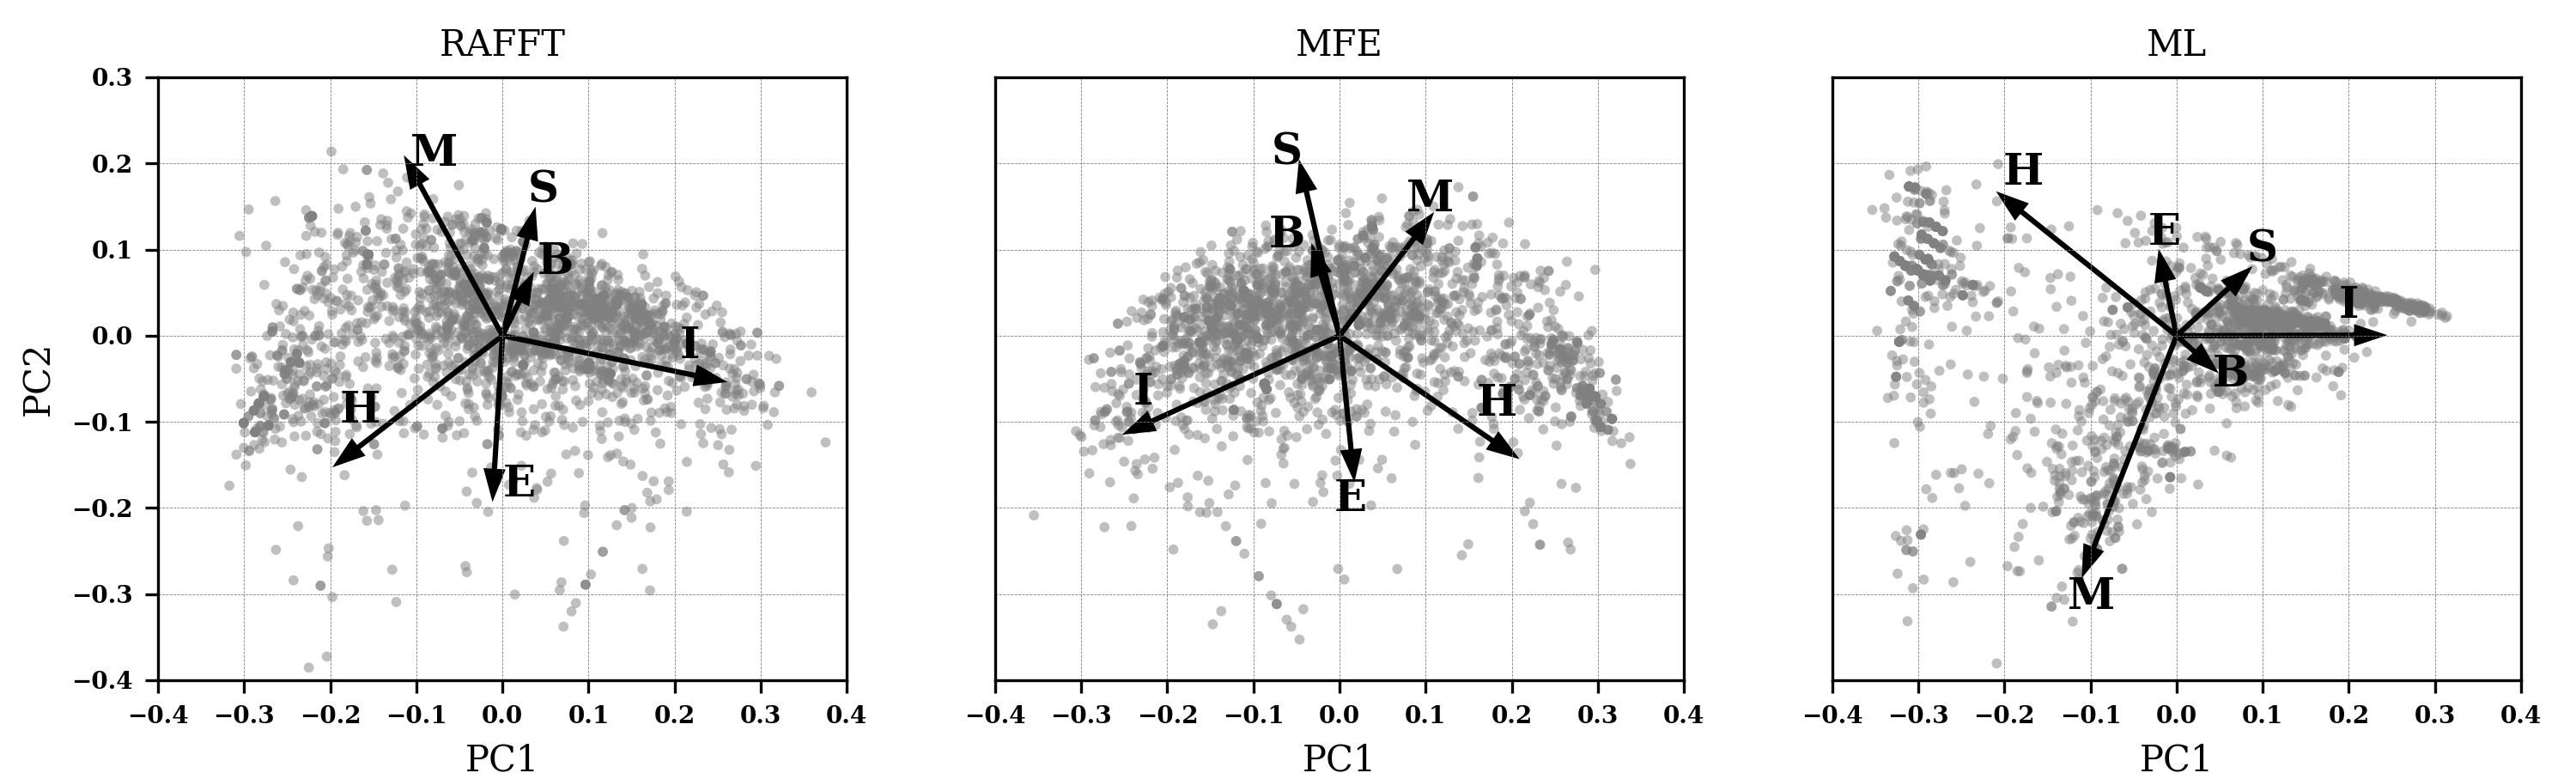
\includegraphics[scale=0.7]{img/pca_predicted.png} 
  \caption{\textbf{PCA analysis of the known structure and predicted
      structures. \label{pca_struct}} The first row shows two PCAs for the known
    structures. In the left side, RAFFT predictions with PPV $\leq$ 10 are
    colored in blue. In the left side, MFE structures with PPV $\leq$ 10 are
    colored in orange. The second row shows the PCA of the predicted strucrures
    for RAFFT, the MFE, and the ML method.}
\end{figure}

\section*{Test case to predict fast-folding paths}
\label{sec:org305ed0a}
Finally, to illustrate RAFFT folding heuristic, we applied it to the Coronavirus
frameshifting stimulation element. It is an RNA sequence of about 82 nucleotides
with a secondary structure determined by sequence analysis and obtained from the
RFAM database. The assumed known structure has a pseudoknot but was not
displayed here. Figure \ref{folding_dynamics} shows the folding path predicted,
the MFE prediction, and the assumed known structure. The approximated
fast-folding paths are predicted in three steps where 5 structures were stored
and 100 positional lags were searched for stems. As shown, some structures
explored were not saved or evolved since no further improvement (relative to all
possibilities) was found. RAFFT was able to recover near-native structures,
found to be closer than the MFE, and depicted simple folding paths. We also
tested with 20 saved structure (see supp. mat.), and obtained similar results.
However, we observed the greediness effect of the algorithm where a better path
in term of stability. Indeed, a better path was achieve since a more stable
structure was found by allowing less stable intermediates.

\begin{figure}[!h]
  \begin{tikzpicture}
    \node (s11) at (0cm,0cm) {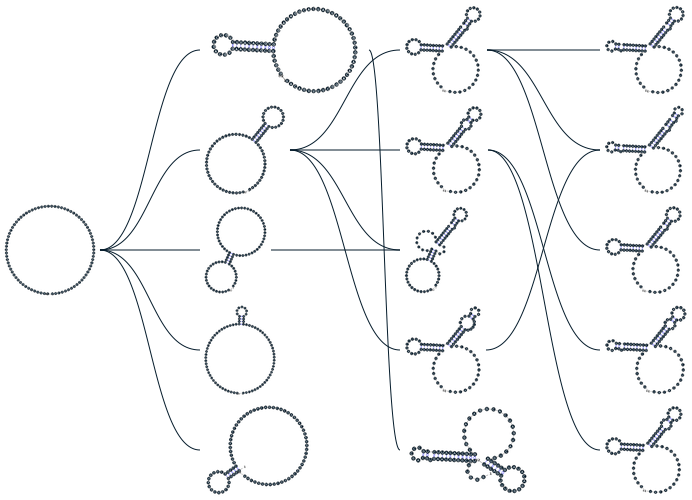
\includegraphics[scale=0.33]{img/frame_shift/path_5.png}};
    \node (wt) at  (9cm,-2cm) {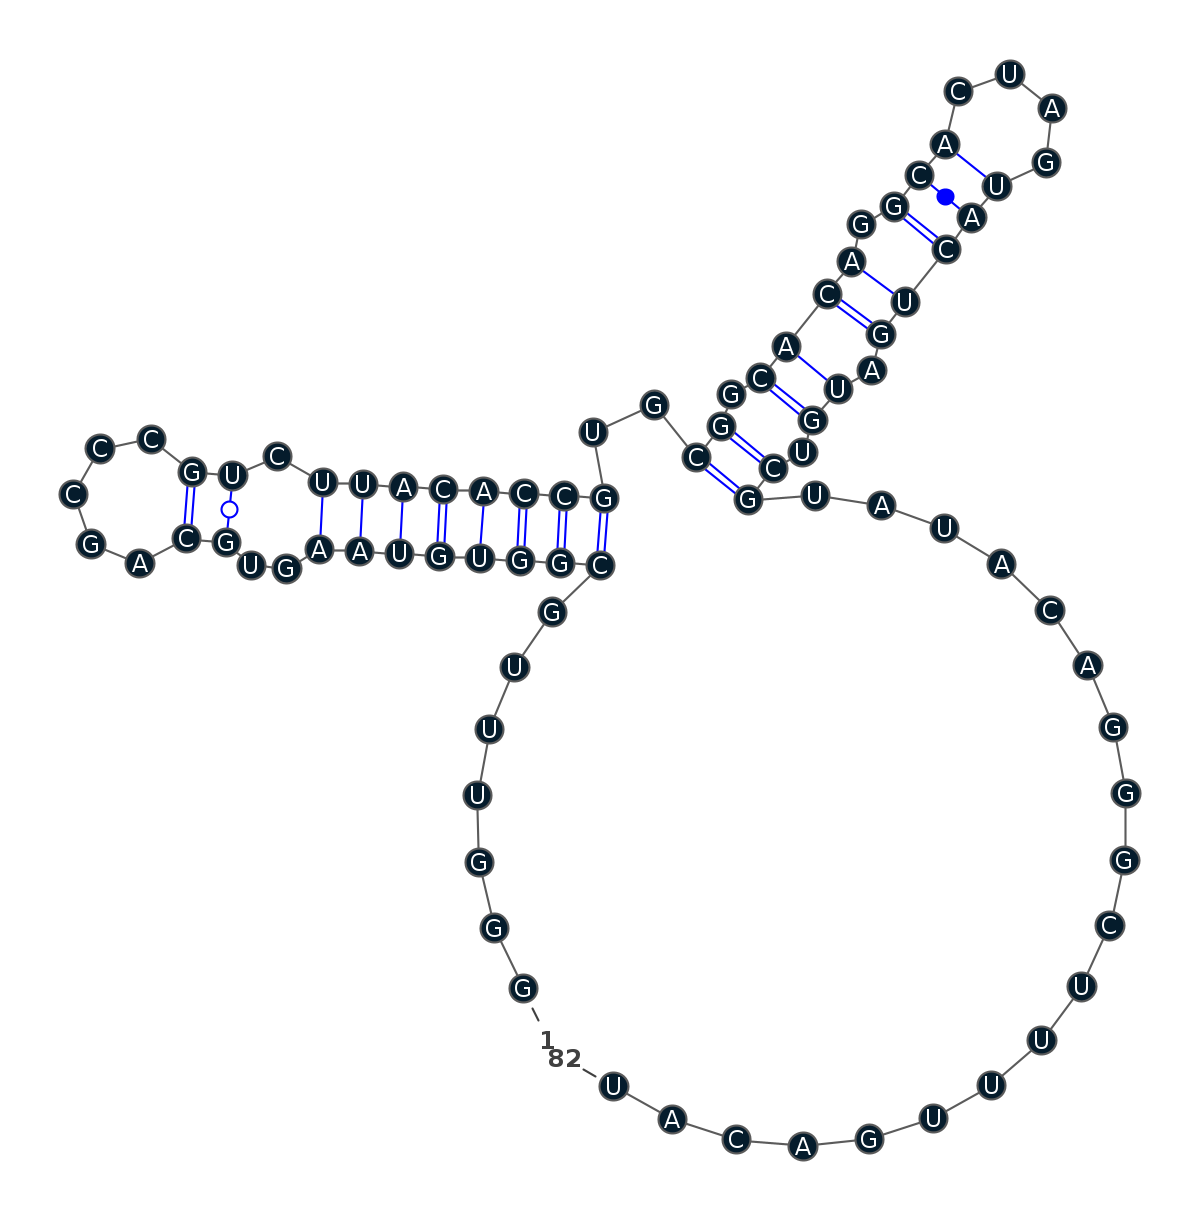
\includegraphics[scale=0.1]{img/frame_shift/wt.png}};
    \node (wtn) at  (8cm,-3cm) {WT};
    \node (mfe) at (9cm,3cm) {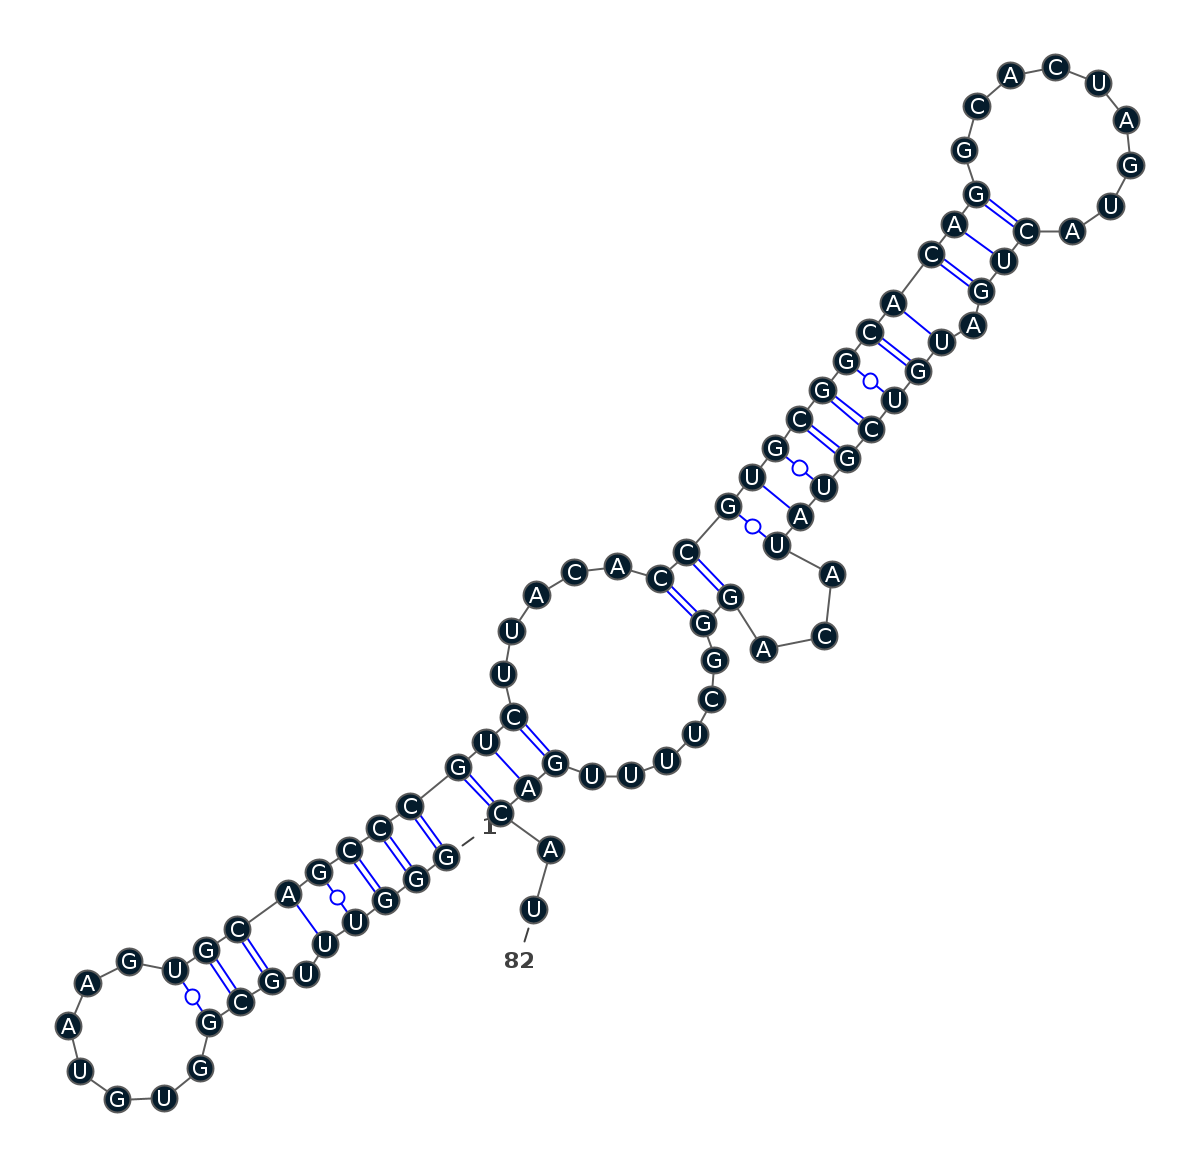
\includegraphics[scale=0.1]{img/frame_shift/mfe.png}};
    \node (mfen) at  (8cm,3cm) {MFE};
  \end{tikzpicture}
  \caption{\textbf{Fast-folding paths prediction for the Coronavirus frameshifting stimulation element.\label{folding_dynamics}.}}
\end{figure}

To visualize the landscape drawn by RAFFT, we produced 300 trajectories with 100
positional lags explored for stems. All unique structures obtained along each
trajectory were mapped onto a plan using the multidimensional scaling (MDS)
algorithm. In the landscape, the MDS optimized the mapping in such a way that
the structure base pair distances were mostly preserved. Figure \ref{landscape}
shows the landscape interpolated with the 751 unique structures found. It
illustrates the two states folding state where all trajectories started from the
high peak in the center, and smoothly roll down to the blue area.


\begin{figure}[h!]
\centering
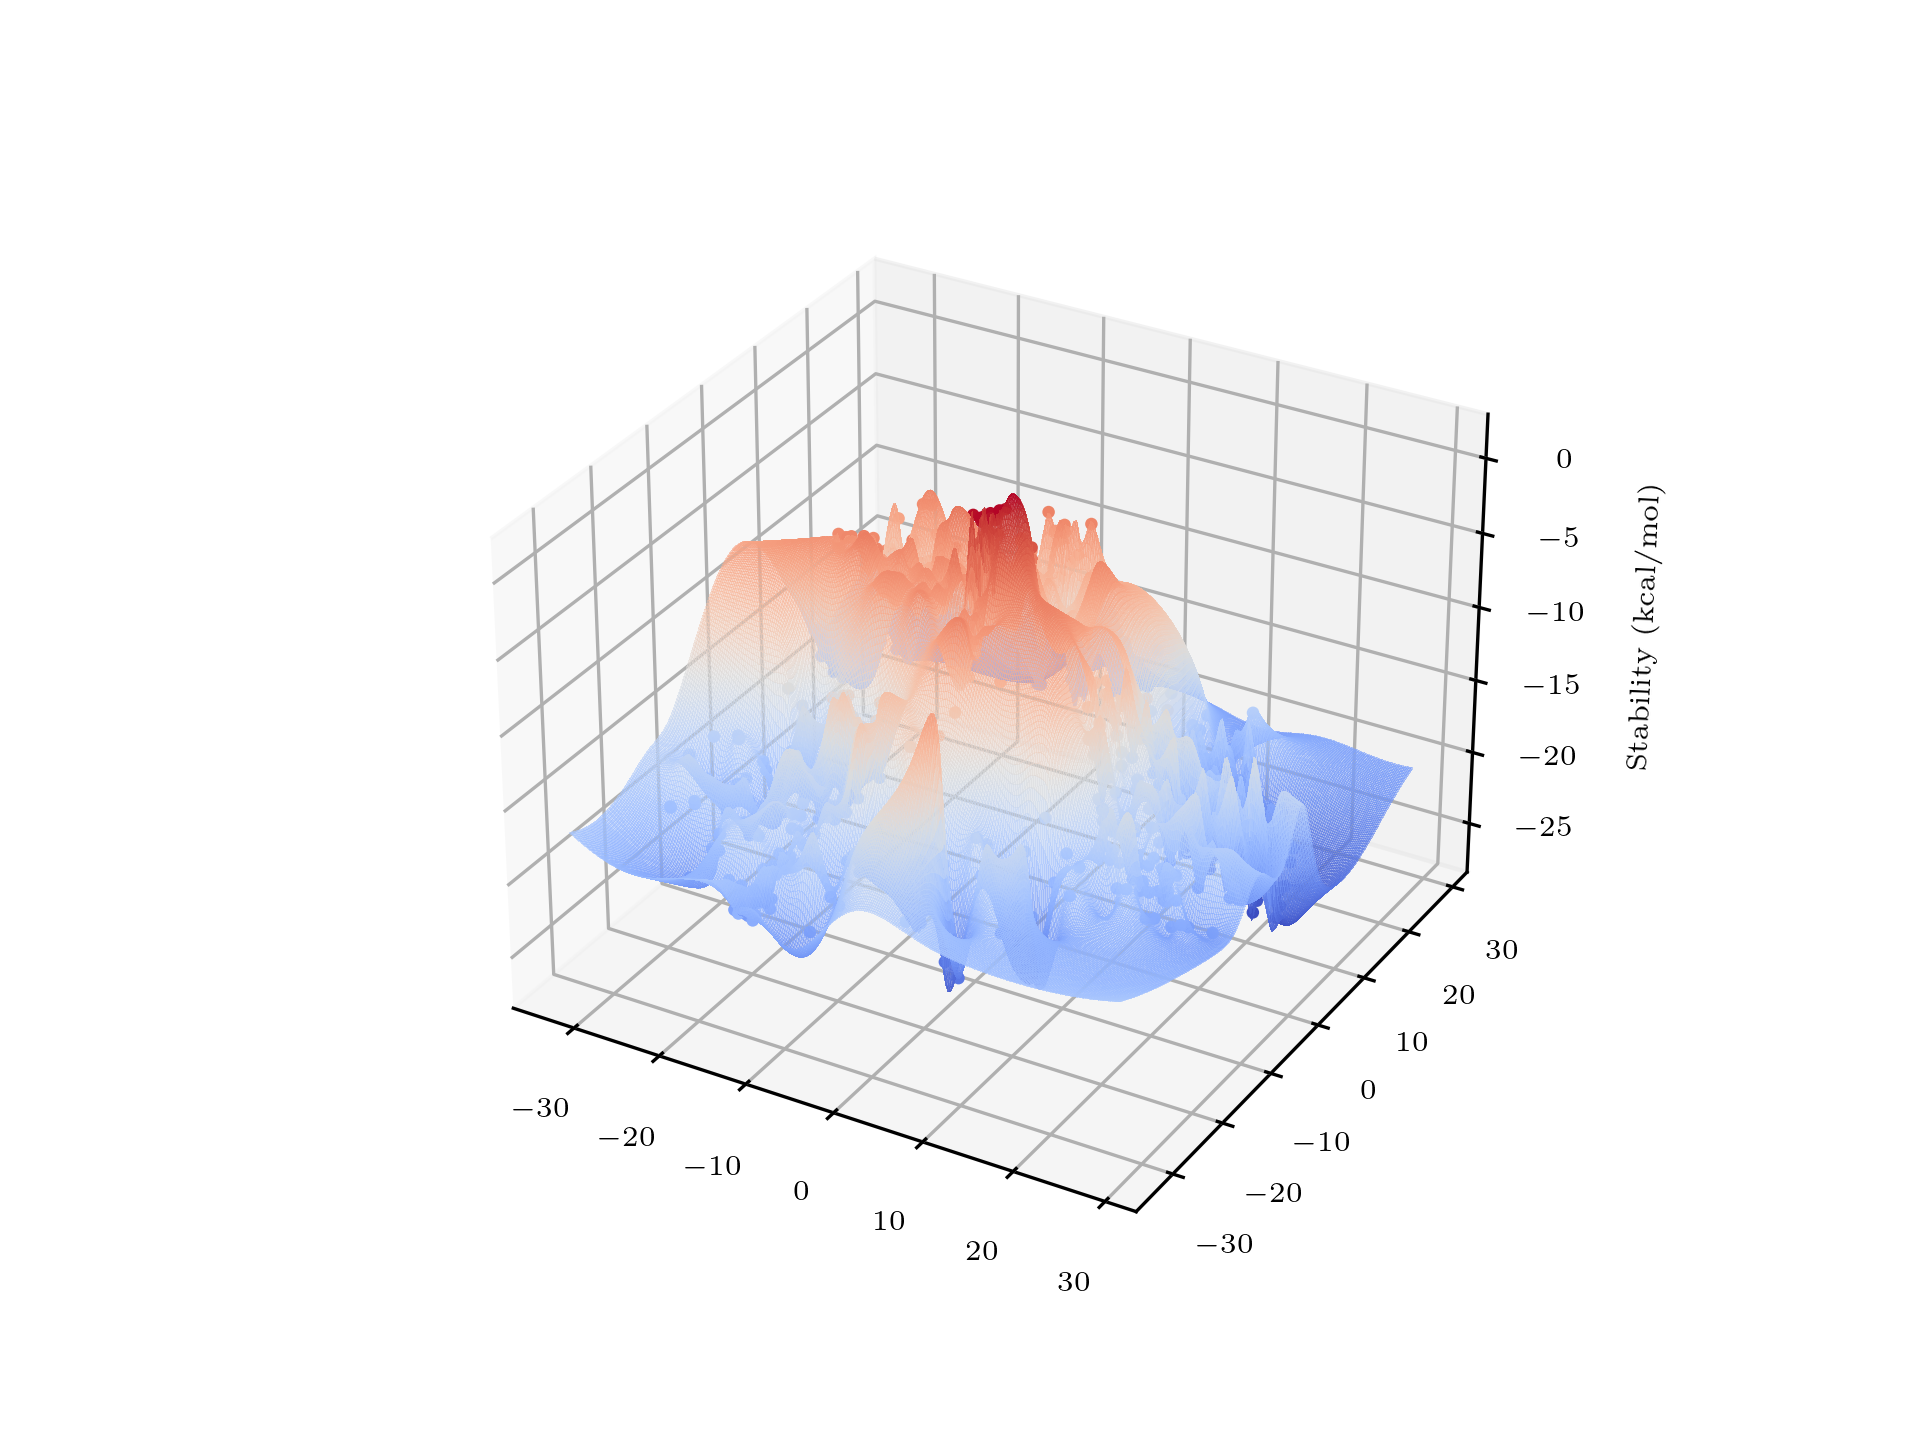
\includegraphics[scale=0.85]{img/landscape.png}
\caption{\label{landscape}\textbf{Landscape built from 300 parallel trajectories.}}
\end{figure}

The graph shown in figure \ref{folding_dynamics} can be use to describe a folding
kinetic where transition can occur from left to right (and right to left) but
not vertically. This follows the idea that parallel paths quickly reach their
end points. However, if the end points are non-native states, it will slowly
fold back into the native state. The kinetic is modeled as a Markov process as
usually done \cite{lorenz20_effic_comput_base_probab_multi_rna_foldin}. The
transition rates \(r(x\rightarowy)\) between structures \(x\) and \(y\) are given by:
\begin{equation}
r(x\rightarrow y) \propto \text{exp}\{-\beta \Delta \Delta G(x\rightarrow y)\}
\end{equation}
where \(\beta=1/kT\) (kcal/mol) is the inverse thermal energy. \(\Delta \Delta
G(x\rightarrow y)\\) is the stability change between structure \(x\) and \(y\). Given
an initial population of only unfolded structures, one can simulate the
evolution of structure populations. The structure 347 which dominates the
kinetic at the end has a stability of -21.0 kcal/mol, and the MFE (also found by
RAFFT) structure has a stability of 25.8 kcal/mol.

\begin{figure}[h!]
\centering
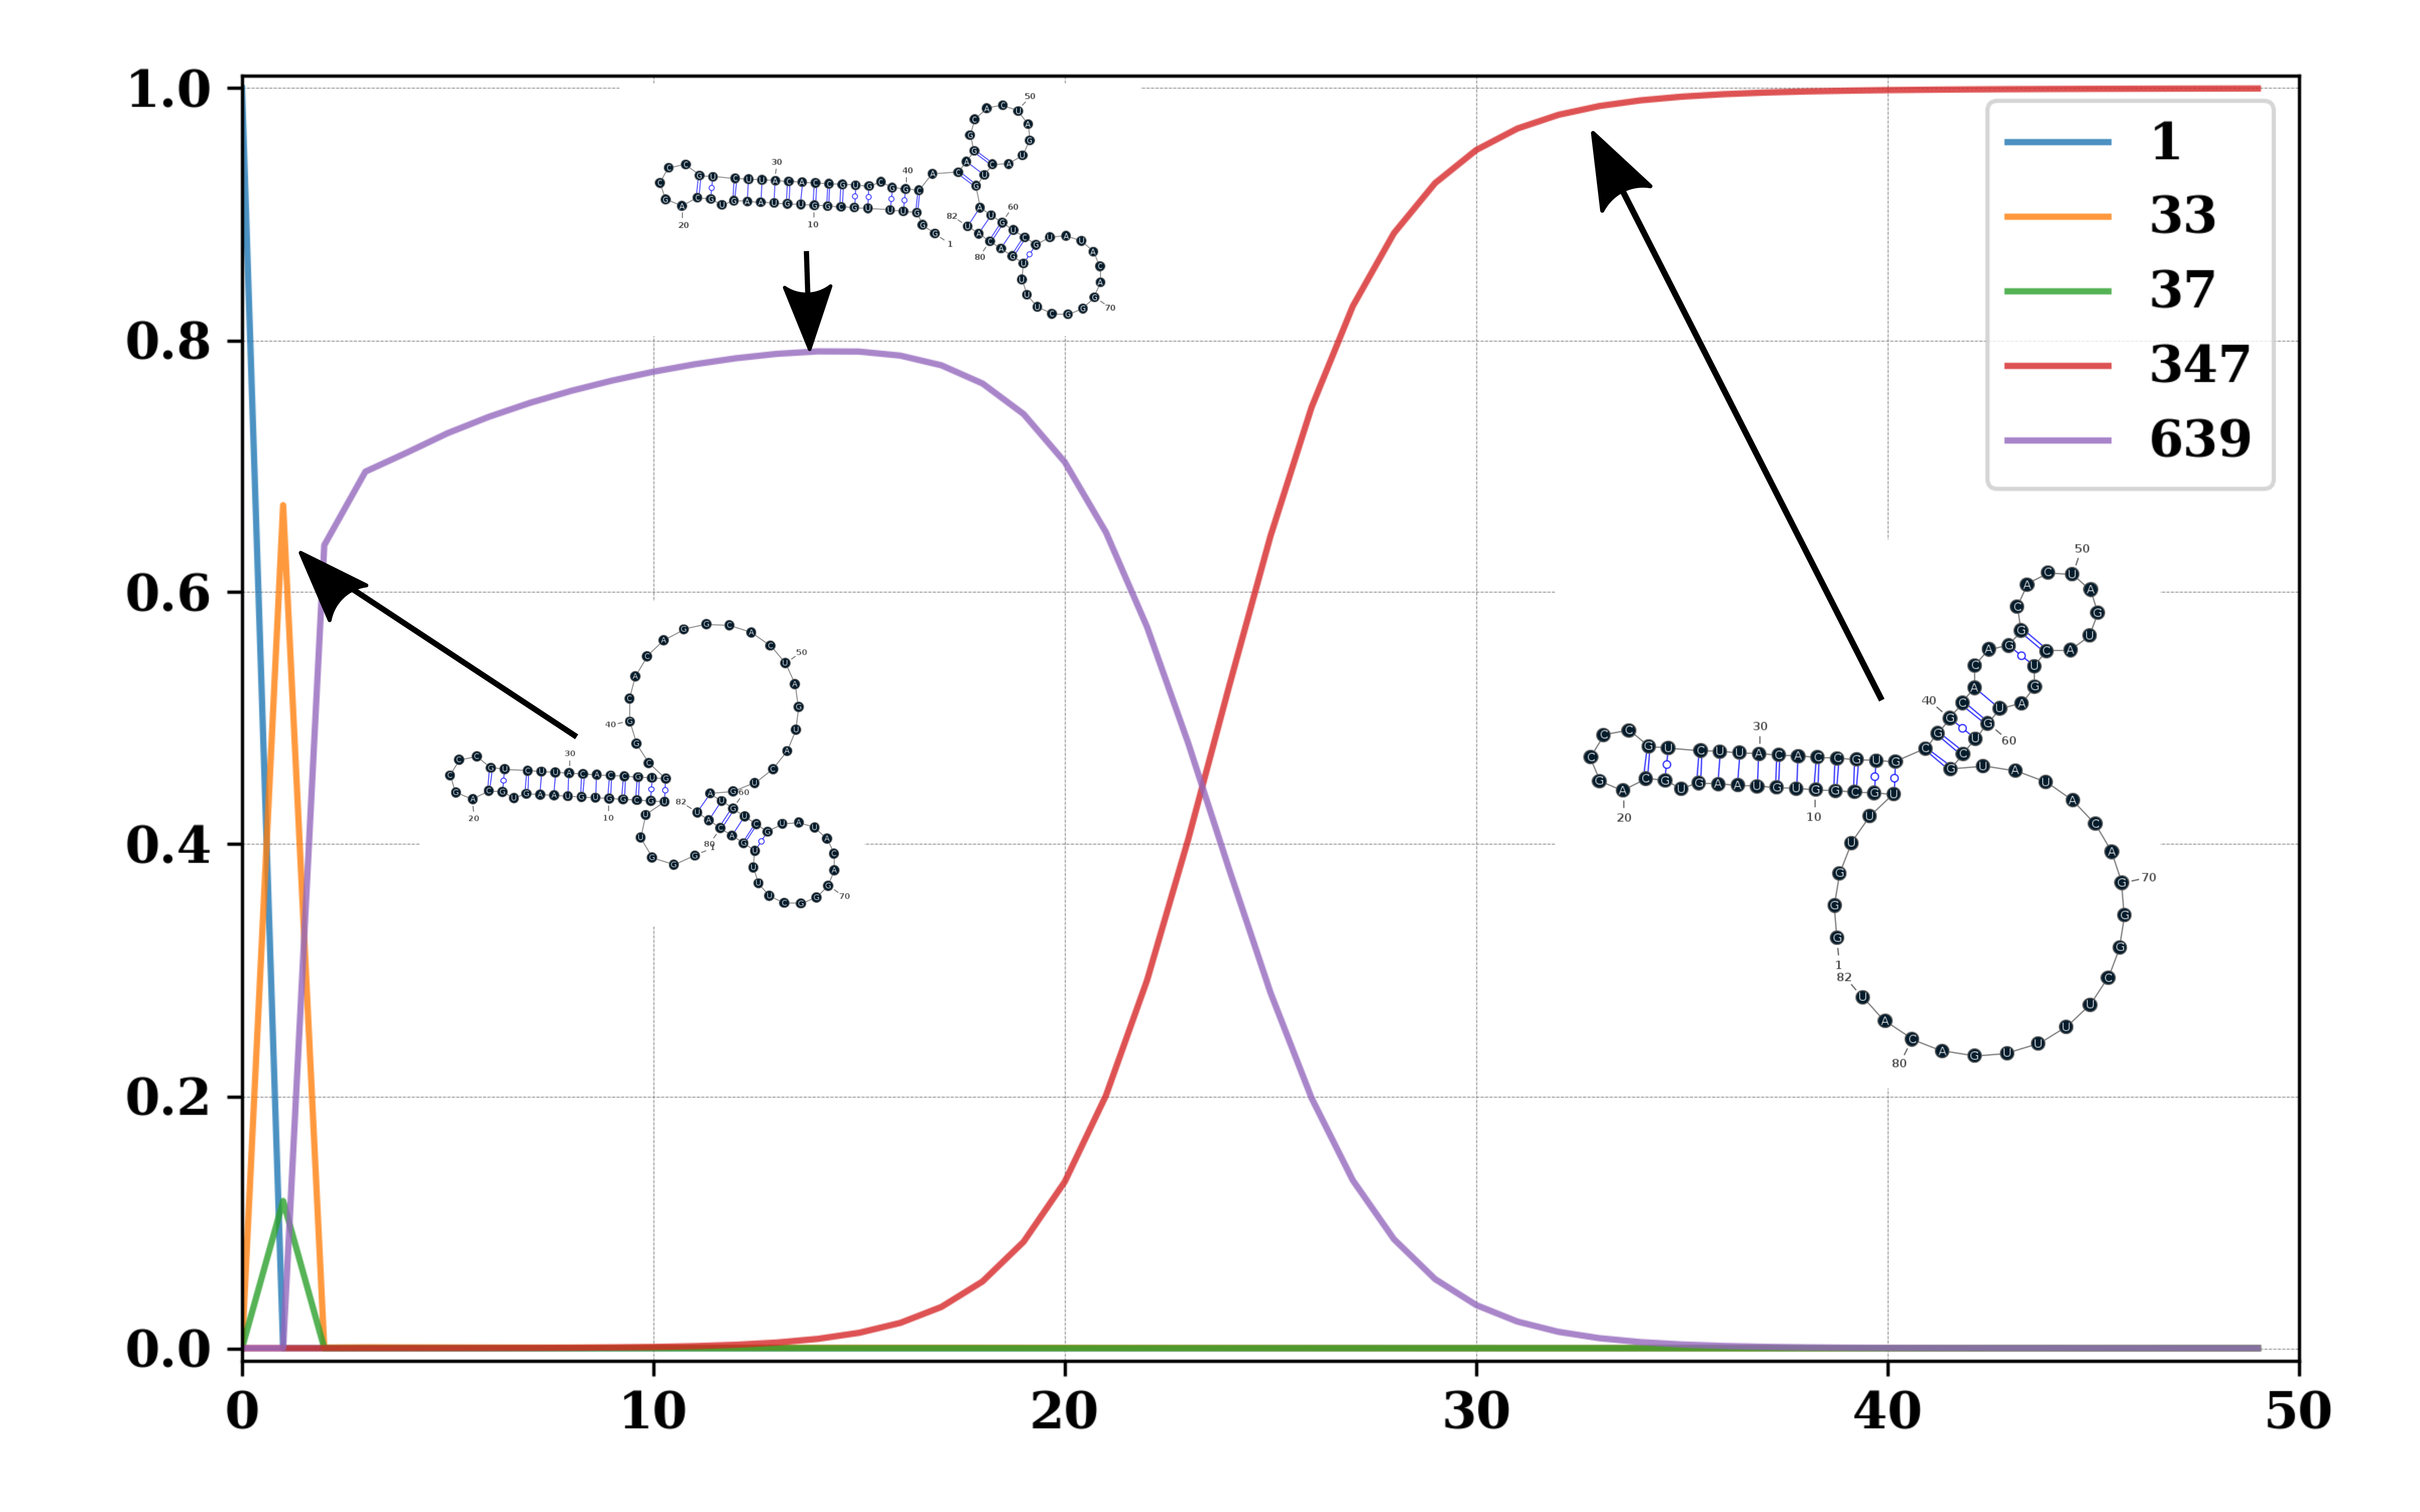
\includegraphics[scale=0.85]{img/kinetic_comb.png}
\caption{\label{landscape}\textbf{Folding kinetic derived from the fast-folding scheme with 300 saved structures.}}
\end{figure}

\section*{Concluding discussion}
\label{sec:org90b93cd}
We have proposed a heuristic of the RNA fast-fold paths called RAFFT. This
heuristic uses a greedy rules. First, it searches for groups of consecutive base
pairs, stems, and from them if they improve the energy. Hence, it produces
smooth and coarse-grained trajectories. To search for consecutive base pairs, we
implemented an FFT-based technique that uses a mirror encoding. Once a stem is
formed, the sequence is split into two independent segments on which one can
recursively search for new stems. For one sequence, the algorithm can follow
multiple folding paths.

To assess the relevance of the folding trajectories produced, we compared the
algorithm performance for the folding task. Two structure estimates were
compared with: the MFE structure computed using RNAfold, the ML-based estimate
using MxFold2. Other thermodynamic-based and ML-based tools were investigated
but not shown here. We chose the MFE since it provides an intuitive
interpretation in the structure landscape, and the MEA prediction was not found
to be significantly more accurate \cite{mathews19_how_to_bench_rna_secon}. The ML
estimates gives a data view of the structure spaces.

From our experiments, RAFFT had an overall performance below the MFE predictions
by 8.1\% of PVV and 10.3\% of sensitivity. The ML-based approach dominated the
predictions (70.4\% of PPV and 77.1\% of sensitivity). We observed some drastic
loss of accuracies when the known structures contained large unpaired regions.
However, those sequences were anecdotal in the dataset. Moreover, those regions
are unlikely to be stable and assumed to be very flexible. Nevertheless, the
effect of unpaired regions seemed less dramatic for the ML method since it can
produce some of those atypical structures. No striking evidences of the length
effect on prediction quality. In addition, no empirical effects of the base
spanning was observed (see supp. mat.) as already pointed out in
\cite{amman13_troub_long_range_base_pairs_rna_foldin}.

The PCA performed on the known structure compositions revealed a structure space
prone to elongated structures where large unpaired hairpin loops and exterior
loops can be observed. The PCA analysis performed on the structures predicted by
the thermodynamic-based methods (RAFFT and MFE) shown similar structure space,
where unpaired regions are of limited number. On the other hand, the ML method
seemed to be closer to the natural structure space. According to the
thermodynamic model, those unpaired regions have local stability equal to zero.
Hence, those regions are not stable at regular experimental conditions in the
sense that they may not have a unique stable structure. However, the ML-method
was able to identify such structure more consistently than thermodynamic
methods. The PCA revealed a group structures with high percents of hairpins.
This may suggest some overfitting effects. Therefore, not being able to recover
such structures would be proof of robustness.

Although the overall performance of RAFFT was only fair compared in the folding
task, we found one among the \(k=50\) predicted trajectories that had better
accuracy than the low energy structure displayed. In fact, the gain of
performance is substantial for the sequences of length below 200 nucleotides
with 16\% better in PPV than the MFE predictions. The performance is
significantly similar to the ML-base method for that length range. Sequences of
length \textless{} 200 nucleotides represent 86.4\% of the total dataset. For the 140
sequences of length greater than 300 nucleotides, all \(k\) predictions per
sequence were similar and performed worst than the other methods. This could be
partially explained by the greediness of the algorithm, however, we also believe
that the thermodynamic energy model could give a complementary explanation.
Indeed, the additivity of the loop contributions to the stability is likely to
be doomed for large sequences \cite{tinoco99_how_rna_folds}. However, the MFE did
not show any notable discrepancy for large sequences (\textgreater{} 300 nucleotides)
except for a few structures with large unpaired regions. This could be explained
by the observation used in kinwalker, where locally optimal substructures
composed the native structures. Therefore, we assume that the MFE structure is
more often composed of locally optimal structures. We tried RAFFT with a larger
number of saved structures in the stack, however, it only got closer to the MFE
prediction quality and did not perform better (see supp. mat.) on large
sequences.

As an illustrative example, we applied the heuristic on a natural RNA, the
Coronavirus frameshifting element. All trajectories started from the unfolded
state to the stable structures in a "two-states" fashion. Furthermore, we showed
that the fast-folding paths model can be used as a kinetic model where
transitions are given by the parallel paths and intermediate structures found.
Because the folding trajectories are already coarse grained and smooth, the
kinetic can be drawn without any additional coarsening. Indeed, usual kinetic
frameworks (\cite{lorenz20_effic_comput_base_probab_multi_rna_foldin}) need a
coarse-grained representation of all attraction basins and the saddle points
that separate them. The structure dominating the kinetic was a structure close
to the native one although lower energy structures where found.

Given the experiment results, we believe that RAFFT is a robust heuristic for
the fast-folding path since it can produce predictions of high accuracy for
86.4\% of this dataset. The folding paths as calculated by RAFFT are smooth and
coarse-grained since whole stems are formed, if it improves the energy, and
leads to near-native structures. This near-native coarse-grained folding path is
an intuitive idea that is similar to the funnel protein folding landscape. We
expect this heuristic to give valuable and complementary information to the
MFE-like predictions. However, additional efforts are necessary to determine
whether the folding paths followed were experimentally observed.

On the technical points, the mirror encoding as describe here is a versatile
tool for RNA analysis. Since it contains the relative positions of base pairs in
the whole sequence, we expect it to be extendable to other use cases such as
sequence clustering, or the speed up of Nussinov-like algorithms. On the other
hand, we are aware of the limits of choosing the maximal number of base pairs
each at each step. However, the greediness of the algorithm had a limited impact
on the results. We are not planning to provide yet another folding tool, in this
already crowded area of excellent software, but one could combine this tool with
an ML-base scoring to discriminate the folding path that is likely to be
observed.

\section*{Methods}
\label{sec:orgaa6074d}
Starting from the ArchiveII dataset, we first removed all the structures with
pseudoknots since all tools considered here don't handle pseudoknots. Next, we
removed all the structures which were evaluated with positive or null energy
with the Turner 2004 energy parameters. Since positive energies mean that the
completely unfolded structure is more stable than the native one. Those
structures are assumed not well modeled by the energy function used here and
therefore would blur the interpretation of the kinetic we try to extract. This
dataset is composed of 2698 structures. 240 sequences were found multiple times
(from 2 to 8 times). 19 of them were found with different structures. We
discarded all duplication and picked the structure with the lowest energy for
each. We obtained a dataset of 2296 sequences.

To compute the MFE structure, we used RNAfold (version) with the default
parameters and the Turner 2004 set of energy parameters. For the machine
learning tool, we computed the prediction using Mxfold2 with the default
parameters. Therefore, only one structure prediction per sequence for those two
methods were used for the statistics.

Two parameters are critical for RAFFT, the number of positional lags in which
stems are searched and the number of saved configurations in the stack. For the
experiments, we search for stems in the 100 best positional lags and stored 50
conformations. For the predictions analysis, we displayed the lowest energy
found at the end for each structure and the most accurate prediction among the
50 saved structures. The correlation which allow to choose the positional lags
was computed using the weights w\textsubscript{GC}=3, w\textsubscript{AU}=2, and w\textsubscript{GU}=1.

To measure the prediction accuracy, we used two metrics from epidemiology. The
positive predictive value (PPV) is the fraction of correct base pairs
predictions in the predicted structure. The sensitivity is the fraction of
correctly predicted base pairs in the true structure. Both metrics are defined
as follow:
\begin{equation}
PPV = \frac{TP}{TP + FN} \;\;\; \text{Sensitivity} = \frac{TP}{TP+FP}
\end{equation}
where TP, FN, and FP stand respectively for the number of correctly predicted
base pairs (true positives), the number of base pairs not detected (false
negatives), and the number of wrongly predicted base pairs (false positives). To
maintain consistency with previous and future studies, we computed these metrics
using the implementation in the \texttt{scorer} tool provided in
\cite{mathews19_how_to_bench_rna_secon}, which provide also a more flexible
estimate where shifts are allowed.

The loop compositions were extracted in terms of percent of the cumulative loop
sizes. This method, although not accurate, gives an overall idea of the
structure space. We first convert the structures into Shapiro notation using
Vienna Package API. From the notation, we extracted the sizes of interior,
exterior, bulge, stacking, hairpins, and multibranch loops. Next, we converted
those sizes into percents of types of loops from which we computed the principal
components. For visual conveniences, the structure compositions were projected
onto the first two principal components. The composition arrows represent the
eigenvectors obtained from the diagonalization of the covariance matrix.

The secondary structure representations were obtained with VARNA
\cite{darty09_varna}.

\bibliographystyle{acm}
\bibliography{d1}
\end{document}
